%%% https://www.overleaf.com/learn is a very good resource for mastering LaTeX

%%% These lines tell the arara program how to compile the document
%%% pdflatex builds the pdf
%%% biber builds the bibliography if you have one
% arara: pdflatex
% arara: biber
% arara: pdflatex
% arara: pdflatex
%%% the following line will tidy up all these extra files that the compiler produces
% arara: clean : {extensions:[aux,bbl,bcf,blg,glg,glo,gls,idx,ilg,ind,ist,lof,lol,lot,nlo,nls,out,ptc,toc,run.xml]}
\documentclass[a4paper, 11pt, extrafontsizes, oneside, openany, x11names]{memoir} % specifies the document class and its options
% You can change 12pt to other sizes
% The memoir class is generally used for writing reports, books, and theses but
% can make any kind of document and looks really nice

%%% The following looks horrible, but essentially sets up biblatex for producing
%%% bibliographies that look nice (you likely will not even need this)
\usepackage[style=authoryear-comp, maxcitenames=2, isbn=false, url=false,
giveninits=true, doi=false, eprint=false, dashed=false, date=year,
related=false, mergedate=true]{biblatex}
\renewbibmacro{in:}{%
  \ifboolexpr{%
     test {\ifentrytype{article}}%
     or
     test {\ifentrytype{inproceedings}}%
  }{}{\printtext{\bibstring{in}\intitlepunct}}%
}
\renewbibmacro*{cite:labelyear+extrayear}{%
  \ifentrytype{online}
    {}
    {\iffieldundef{labelyear}
      {}
      {\printtext[bibhyperref]{%
         \printfield{labelyear}
         \printfield{extrayear}}}}}

\AtEveryBibitem{%
  \clearfield{pagetotal}%
}

\DeclareFieldFormat[article,inbook,incollection,techreport,inproceedings,patent,thesis,unpublished]{title}{#1\isdot}
\DeclareFieldFormat{pages}{#1}


\usepackage{caption}
\usepackage{subcaption}

\usepackage{amsbsy} % for producing bold maths symbols
\usepackage{amsfonts} % an extended set of fonts for maths
\usepackage{amssymb} % various maths symbols
\usepackage{amsthm} % for producing theorem-like environments
\usepackage{array} % for nice array and tabular environments
\usepackage{datetime2} % managing dates and times
\usepackage{delimseasy} % makes easy the manual sizing of brackets, square brackets, and curly brackets
\usepackage{enumitem} % customing list environments
\usepackage{float} % makes dealing with floats (e.g. tables and figures) easier
\usepackage{framed} % for producing framed boxes
\usepackage{graphicx} % for including graphics in the document
\usepackage{hyperref} % automatically produce hyperlinks for cross-references
\usepackage{mathtools} % package for maths (fixes some deficiences of amsmath so is preferred)
\usepackage{cleveref} % makes cross-referencing easier (must be loaded after hyperref and mathtools)
\usepackage{microtype} % better font sizing (extremely helpful with long equations!)
\usepackage{newtx} % a fonts package
\usepackage{pdfpages} % for including pdf documents inside the compiled pdf
\usepackage{pgf} % produce pdf graphics using LaTeX
\usepackage{pgfplots} % create normal/logarithmic plots in two and three dimensions
\pgfplotsset{compat=1.18} % sorts out the compatability warning
\usepackage{physics} % useful for vector calculus and linear algebra symbols
\usepackage[theorems]{tcolorbox} % for producing coloured boxes
\tcbuselibrary{theorems} % theorems with tcolorbox
\usepackage{tikz-3dplot} % for producing 3d plots
\usepackage{tikz} % for drawing graphics in LaTeX
\usepackage{tkz-base} % drawing with a Cartesian coordinate system
\usepackage{tkz-euclide} % drawing in Euclidean geometry

\usepackage{pifont}
\DeclareMathAlphabet{\mathcal}{OMS}{cmsy}{m}{n}

\definecolor{myblack}{RGB}{0, 0, 0}
\definecolor{mywhite}{RGB}{255, 255, 255}
\definecolor{mylightblue}{RGB}{102, 178, 255}
\definecolor{mymidblue}{RGB}{0, 128, 255}
\definecolor{mydarkblue}{RGB}{0, 0, 204}
\definecolor{mylightgreen}{RGB}{0, 255, 128}
\definecolor{mymidgreen}{RGB}{0, 204, 102}
\definecolor{mydarkgreen}{RGB}{0, 153, 0}
\definecolor{mylightred}{RGB}{255, 51, 51}
\definecolor{mymidred}{RGB}{204, 0, 0}
\definecolor{mydarkred}{RGB}{153, 0, 0}
\definecolor{myyellow}{RGB}{255, 255, 0}
\definecolor{myorange}{RGB}{255, 153, 51}
 % imports the packages.tex file from the preamble directory
%%% Everything below sets up the environments
\tcbset{%
  defstyle/.style={colframe=mydarkblue, colback=mylightblue, colbacktitle=mymidblue,%
    coltitle=myblack, colupper=myblack, toprule=1mm, bottomrule=1mm,%
    leftrule=1mm, rightrule=1mm},
  theostyle/.style={colframe=mydarkgreen, colback=mylightgreen, colbacktitle=mymidgreen,%
    coltitle=myblack, colupper=myblack, toprule=1mm, bottomrule=1mm,%
    leftrule=1mm, rightrule=1mm},
  assstyle/.style={colframe=myorange, colback=mylightred, colbacktitle=mymidred,%
    coltitle=myblack, colupper=myblack, toprule=1mm, bottomrule=1mm,%
    leftrule=1mm, rightrule=1mm},
  exestyle/.style={colframe=cyan, colback=mylightblue, colbacktitle=mymidblue,%
    coltitle=myblack, colupper=myblack, toprule=1mm, bottomrule=1mm,%
    leftrule=1mm, rightrule=1mm},
  exastyle/.style={colframe=myorange, colback=myyellow, colbacktitle=myyellow,%
    coltitle=myblack, colupper=myblack, toprule=1mm, bottomrule=1mm,%
    leftrule=1mm, rightrule=1mm},
  conjstyle/.style={colframe=olive, colback=myyellow, colbacktitle=myyellow,%
    coltitle=myblack, colupper=myblack, toprule=1mm, bottomrule=1mm,%
    leftrule=1mm, rightrule=1mm},
  remstyle/.style={colframe=lime, colback=mylightgreen, colbacktitle=mymidgreen,% 
    coltitle=myblack, colupper=myblack, toprule=1mm, bottomrule=1mm%,
    leftrule=1mm, rightrule=1mm}
}

\newtcbtheorem[number within=section, Crefname={definition}{definitions}]{definition}{Definition}{defstyle}{def}
\newtcbtheorem[number within=section, Crefname={theorem}{theorems}]{theorem}{Theorem}{theostyle}{theo}
\newtcbtheorem[number within=section, Crefname={assumption}{assumptions}]{assumption}{Assumption}{assstyle}{ass}
\newtcbtheorem[number within=section, Crefname={exercise}{exercises}]{exercise}{Exercise}{exestyle}{exe}
\newtcbtheorem[number within=section, Crefname={example}{examples}]{example}{Example}{exastyle}{exa}
\newtcbtheorem[number within=section, Crefname={conjecture}{conjectures}]{conjecture}{Conjecture}{conjstyle}{conj}
\newtcbtheorem[number within=section, Crefname={remark}{remarks}]{remark}{Remark}{remstyle}{rem}
\newtcbtheorem[use counter from=theorem, Crefname={corollary}{corollaries}]{corollary}{Corollary}{theostyle}{cor}
\newtcbtheorem[use counter from=theorem, Crefname={lemma}{lemmas}]{lemma}{Lemma}{theostyle}{lem}
\newtcbtheorem[use counter from=theorem, Crefname={proposition}{propositions}]{proposition}{Proposition}{theostyle}{prop}
\newtcbtheorem[use counter from=conjecture, Crefname={question}{questions}]{question}{Question}{conjstyle}{conj}
\newtcbtheorem[use counter from=conjecture, Crefname={speculation}{speculations}]{speculation}{Speculation}{conjstyle}{spec}

\tcolorboxenvironment{proof}{colframe=mydarkred, colback=mylightred,%
colbacktitle=mymidred, coltitle=myblack, colupper=myblack, toprule=1mm,%
bottomrule=1mm, leftrule=1mm, rightrule=1mm}
 % imports the environments.tex file from the preamble directory
% General writing
\newcommand{\bracket}[1]{\left(#1\right)} % for automatic resizing of brackets
\newcommand{\sbracket}[1]{\left[#1\right]} % for automatic resizing of square brackets
\newcommand{\mset}[1]{\left\{#1\right\}} % for automatic resizing of curly brackets
\newcommand{\defeq}{\coloneqq} % the "defined as" command
\newcommand{\ndash}{--\ } % for producing a dash
\newcommand{\mdash}{---\ } % for producing a longer dash
\newcommand{\by}{\times} % used for talking about m by n matrices
\newcommand{\eg}{e.g.\ } % for example
\newcommand{\ie}{i.e.\ } % i.e.
\newcommand{\RNum}[1]{\uppercase\expandafter{\romannumeral #1\relax}} % uppercase roman numerals
\renewcommand{\cite}{\textcite} % easier citing
\newcommand{\hide}[1]{} % useful for temporarily removing some code

\newcommand{\rednote}[1]{{\color{red} #1}} % for red text
\newcommand{\bluenote}[1]{{\color{blue} #1}} % for blue text
\newcommand{\greennote}[1]{{\color{green} #1}} % for green text

% Blackboard Maths Symbols
\newcommand{\N}{\mathbb{N}} % natural numbers
\newcommand{\Q}{\mathbb{Q}} % rational numbers
\newcommand{\Z}{\mathbb{Z}} % integers
\newcommand{\R}{\mathbb{R}} % real numbers
\newcommand{\C}{\mathbb{C}} % complex numbers
\newcommand{\E}{\mathbb{E}} % expectaion operators
\renewcommand{\P}{\mathbb{P}} % probability measures

% Calligraphic Maths Symbols
\newcommand{\F}{\mathcal{F}} % sigma-field

% Bold Maths Symbols
\newcommand{\1}{\mathbf{1}} % characteristic function

% Maths operations
\newcommand{\union}{\cup} % union
\newcommand{\intersect}{\cap} % intersection
\newcommand{\directsum}{\oplus} % direct sum
\newcommand{\Union}{\bigcup} % bigger union symbol
\newcommand{\Intersect}{\bigcap} % bigger intersection symbol
\newcommand{\Directsum}{\bigoplus} % bigger direct sum symbol
\newcommand{\tensor}{\otimes} % tensor
\newcommand{\Tensor}{\bigotimes} % bigger tensor symbol
\newcommand{\remove}{\setminus} % set difference
\renewcommand{\hom}[2]{\operatorname{Hom}\bracket{{#1}, {#2}}} % Hom sets

% Maths operations
\newcommand{\powerset}[1]{\mathcal{P}\bracket{#1}} % powerset
\renewcommand{\ip}[3]{\left \langle #1, #2 \right \rangle_{#3}} % inner product
\newcommand{\cardinality}[1]{\operatorname{Card}\bracket{#1}} % cardinality
\newcommand{\inv}[1]{#1^{-1}} % inverse
\newcommand{\adj}[1]{#1^{*}} % adjoint
\newcommand{\conj}[1]{\overline{#1}} % conjugate
\newcommand{\vspan}[1]{\operatorname{Span}\left\{#1\right\}} % vector space span
\renewcommand{\rank}[1]{\operatorname{Rank}\bracket{#1}} % rank of a linear transformation
\newcommand{\diag}[1]{\operatorname{Diag}\bracket{#1}} % diagonal elements of a square matrix
\renewcommand{\tr}[1]{\operatorname{Tr}\bracket{#1}} % trace
\newcommand{\kernel}[1]{\operatorname{Ker}\bracket{#1}} % kernel
\newcommand{\im}[1]{\operatorname{Im}\bracket{#1}} % image
\newcommand{\range}[1]{\operatorname{Ran}\bracket{#1}} % range
\newcommand{\col}[1]{\operatorname{Col}\bracket{#1}} % column space
\renewcommand{\exponential}[1]{\operatorname{exp}\bracket{#1}} % exponential function
\newcommand{\floor}[1]{\left\lfloor#1\right\rfloor} % macro for the floor function
\renewcommand{\ceil}[1]{\left\lceil#1\right\rceil} % macro for the ceiling function
\newcommand{\dx}{\,\mathrm{d}x} % differential of x
\newcommand{\dy}{\,\mathrm{d}y} % differential of y
\newcommand{\dt}{\,\mathrm{d}t} % differential of t


% optimisation objectives
\DeclareMathOperator*{\argmin}{argmin} % argument which minimises some criterion
\DeclareMathOperator*{\argmax}{argmax} % argument which maximises some criterion
\DeclareMathOperator*{\arginf}{arginf} % argument that gives the infimum of some criterion
\DeclareMathOperator*{\argsup}{argsup} % argument that gives the supremum of some criterion

% Statistical operations
\newcommand{\given}{\vert} % given (used in conditional probability)
\newcommand{\suchthat}{\;\middle|\;} % such that
\newcommand{\probspace}{\bracket{\Omega, \F, \P}} % a probability space
\newcommand{\borel}[1]{\B\bracket{#1}} % the Borel sigma-field
\newcommand{\prob}[1]{\P\bracket{#1}} % Probability
\newcommand{\cprob}[2]{\P\bracket{#1 \middle\given #2}} % Conditional probability
\newcommand{\expect}[1]{\E\bracket{#1}} % Expectation
\newcommand{\cexpect}[2]{\E\bracket{#1 \middle\given #2}} % Conditional expectation
\renewcommand{\var}[1]{\operatorname{Var}\bracket{#1}} % Variance
\newcommand{\cvar}[2]{\operatorname{Var}\bracket{#1 \middle\given #2}} % Conditional variance
\newcommand{\cov}[2]{\operatorname{Cov}\bracket{#1, #2}} % Covariance
\newcommand{\ccov}[3]{\operatorname{Cov}\bracket{#1, #2 \middle\given #3}} % Conditional covariance
\newcommand{\corr}[2]{\operatorname{Corr}\bracket{#1, #2}} % Correlation
\newcommand{\ccorr}[3]{\operatorname{Corr}\bracket{#1, #2 \middle\given #3}} % Conditional correlation

% Statistical symbols
\newcommand{\indep}{\perp\!\!\!\!\!\perp} % statistical independence
\newcommand{\sigfield}[1]{\sigma\bracket{#1}} % sigma-field
\newcommand{\evalue}[1]{\lambda_{#1}} % eigenvalue
 % imports the macros.tex file from the preamble directory
\setlength{\parindent}{0.2in} % sets the size of paragraph indenting
\setlength{\parskip}{0pt} % sets the size of the gap between paragraphs
\setlength{\abovedisplayskip}{3pt} % sets the size of the gap induced by \abovedisplayskip
\setlength{\belowdisplayskip}{3pt} % similar
\setlength{\abovedisplayshortskip}{0pt} % similar
\setlength{\belowdisplayshortskip}{0pt} % similar
\linespread{1.0} % spacing between lines
\setcounter{tocdepth}{3} % how many levels of sectioning will go into the table of contents
\setsecnumdepth{subsubsection} % numbers subsubsection environments
\allowdisplaybreaks[1] % stops forcing pagebreaks before very long align environments
\nouppercaseheads % stops headers being made entirely uppercase

%%% Sets up the page layout
\makepagestyle{contents}
\makeevenhead{contents}{\itshape \rightmark}{}{}
\makeoddhead{contents}{\itshape \rightmark}{}{}
\makeevenfoot{contents}{}{\thepage}{}
\makeoddfoot{contents}{}{\thepage}{}
 % imports the settings.tex file from the preamble directory

\addbibresource{bib/library.bib} % this is your list of references (you can use Zotero to organise your references and generate a bib file)

%%%%%%%%%%%%%%%%%%%%%%%%%%%%%%%%%%%%%%%%%%%%%%%%%%%%%%%%%%%%%%%%%%%%%%%%%%%%%%%%%%%%%%%%%%%%%%%%%%%%%%%%%%%%%%%%%%%%%%%%%%%%%%%%%%%%%%%%%%%
\begin{document} % starts the document

\frontmatter % formats the stuff before the main document begins
\begin{titlingpage*}
   \begin{center}
       \vspace*{5cm}

       {\HUGE Machine Learning}
       
       \vspace{3cm}

       {\LARGE Andrea Sanchietti}
    

       \vspace{5cm}

       {\Large 2022/2023}
   \end{center}
\end{titlingpage*}
 % imports the titlepage.tex file from the preamble directory
\clearpage % starts a new page
\pagestyle{contents} % specifies how to format the table of contents
\tableofcontents* % produces the table of contents
\clearpage % starts a new page

\mainmatter % formats the main document
\chapter{Classification Evaluation}\label{chapter1} % begins a chapter and labels it for cross-referencing
\section{Classification Evaluation}\label{ClassificationEvaluation} % start a new section and label it for cross-referencing

\subsection{Performance evaluation}

Performance evaluation in classification is based on \emph{accuracy} and \emph{error rate}.

Consider a typical classification problem:
\begin{equation}
    f: X \xrightarrow{} Y \\
\end{equation}
$\mathcal{D}$: probability distribution over X \\
$\mathcal{S}$: sample of n instances drawn from X \\
Consider a hypothesis h, solution of a learning algorithm obtained from S. What is the best estimate of the accuracy of h over future instances drawn from the same distribution? What is the probable error in this accuracy estimate?

\subsubsection{true error and sample error}
    true error of hypothesis h with respect to target function f and distribution D is the probability that h will misclassify an instance drawn at random according to D
\begin{equation}
    error_{\mathcal{D}}(h) \equiv \prod_{x \in D} [\sigma (f(x) \neq h(x))]
\end{equation}
The sample error of h with respect to target function f and data sample
S is the proportion of examples h misclassifies
\begin{equation}
    error_{\mathcal{S}}(h) \equiv \frac{1}{n}\sum_{x \in S} \sigma (f(x) \neq h(x))
\end{equation}
where $\sigma (f(x) \neq h(x))$ is equal to 1 if $f(x) \neq h(x)$ and 0 otherwise.

Note: $accuracy(h) = 1 - error(h)$

The true error cannot be computed, the sample error is computed only
on a small data sample.

If $accuracyS (h)$ is very high, but $accuracyD(h)$ is poor, then our system
would not be very useful.

\subsubsection{Estimating Bias}

\begin{equation}
    bias = E[error_S (h)] - error_D (h)
\end{equation}

\subsubsection{Confidence interval}
with approximate N\% probabiliry, $error:D (h)$ lies in interval
\begin{equation}
    error_S (h) +- z_{N} \sqrt{\frac{error_S(h) (1-error_S(h))}{n}}
\end{equation}
where
\begin{figure}[H]
    \centering
    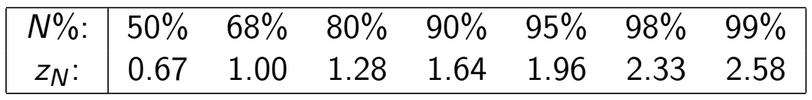
\includegraphics[width=12cm,keepaspectratio]{images/Classification Evaluation/Screenshot_20221004_125528.png}
    \caption{Value of z$_{N}$  based on the $N\%$ chosen}
    \label{fig:z_N}
\end{figure}

\subsubsection{K-Fold Cross Validation}

Partition data set D into k disjoint sets $S_1, S_2, . . . , S_k (|S_i| > 30)$ and then use one set as test set while the remaining sets as training set

The error is
\begin{equation}
    error_{L,D} \equiv \frac{1}{k}\sum_{i = 1}^{k}\sigma_i
\end{equation}

note: $accuracy_{L,D} = 1 - error_{L, D}$

\subsubsection{Comparing learning algorithms}

If we have two hypothesis $h_1, h_2$, the true comparison is
\begin{equation}
    d \equiv error_D (h_1) - error_D (h_2)
\end{equation}

and its estimator is

\begin{equation}
    \hat{d} \equiv error_{S_1} (h_1) - error_{S_2} (h_2)
\end{equation}

$\hat{d}$ is an unbiased estimator for d, iff $h_1, h_2, S_1 and S_2$ are independent from each other
\begin{equation}
    E[\hat{d}] = d
\end{equation}

to estimate which algorithm is better we would like to estimate:
\begin{equation}
    E_{S\subset D}[error_D (L_A(S)) - error_D(L_B(S))]
\end{equation}

where L(S) is the hypothesis output by learner L using training set S

this measure can be approximated by K-Fold cross validation

\subsection{Performance Metrics}

\begin{figure}[H]
    \centering
    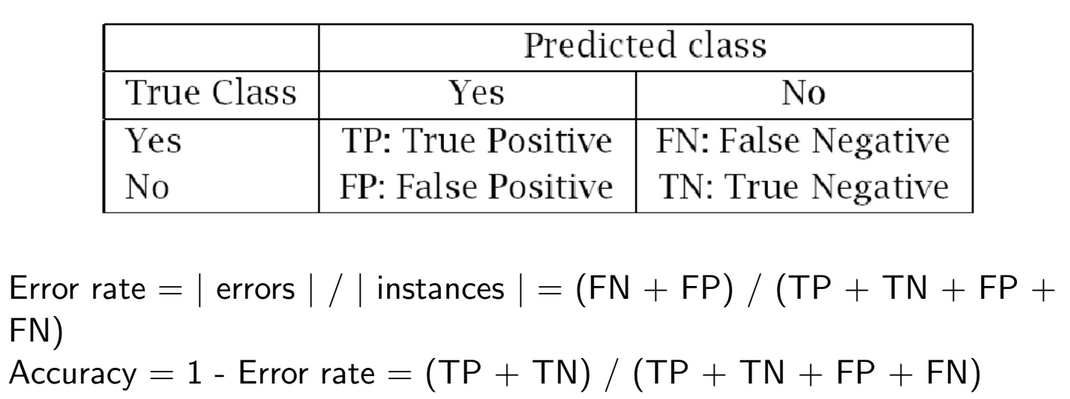
\includegraphics[width=12cm,keepaspectratio]{images/Classification Evaluation/Screenshot_20221004_131728.png}
    \caption{}
    \label{fig:image2}
\end{figure}

Sometimes accuracy is not enough. Imagine a dataset of 90 cats and 10 dogs. An algorithm that always returns "cat" will have 90$\%$ accuracy while a classification algorithm may have 85$\%$, but actually be good.

Unbalanced data sets are very common in problems related to anomaly detection.

Other Performance metrics are:

\begin{figure}[H]
    \centering
    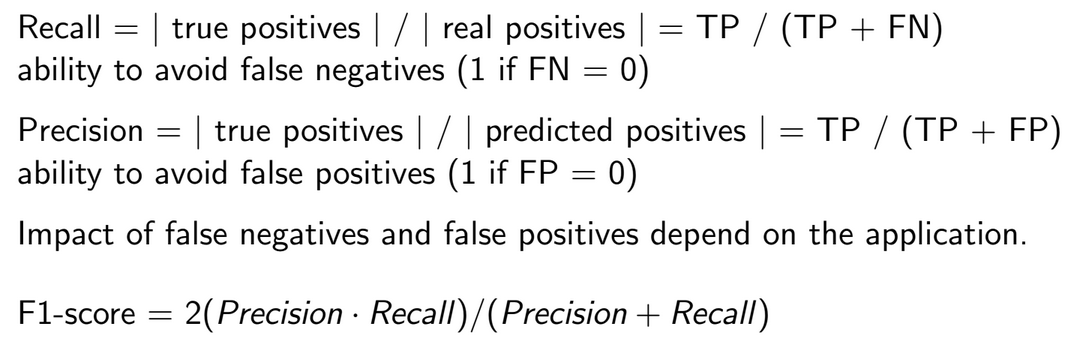
\includegraphics[width=12cm,keepaspectratio]{images/Classification Evaluation/Screenshot_20221004_134809.png}
    \caption{}
    \label{fig:image_metric_1}
\end{figure}

\begin{figure}[H]
    \centering
    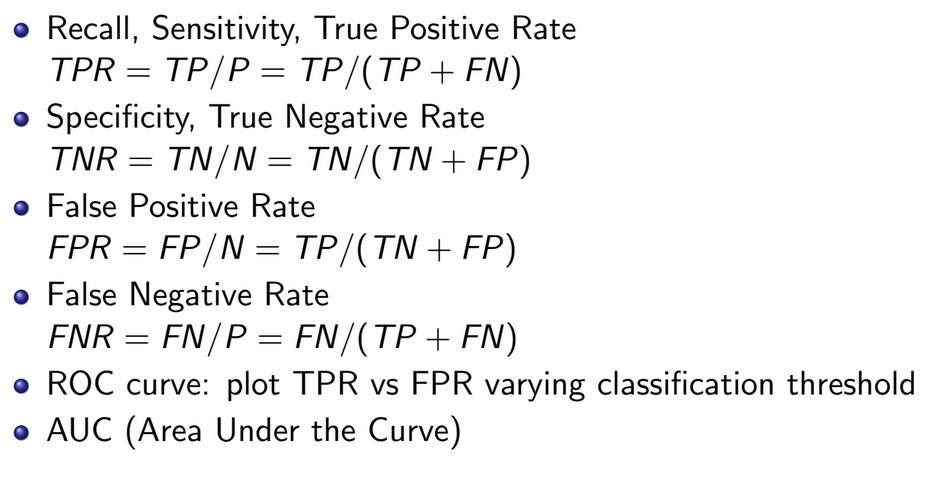
\includegraphics[width=12cm,keepaspectratio]{images/Classification Evaluation/Screenshot_20221004_135110.png}
    \caption{}
    \label{fig:image_metric_2}
\end{figure} % imports the section1.tex file from the chapters/chapter1 directory

\newpage

\chapter{Decision Trees}
\section{Decision Trees}\label{DecisionTrees} % start a new section and label it for cross-referencing

\subsection{The problem}
Problem: Given a training set D for a target function c, compute the ”best” consistent hypothesis wrt D.


Consider a discrete input space described with $m$ attributes $X = A_1 \times \dots \times A_m$ with A$_{i}$ finite, and a classification problem for f: X $\xrightarrow[]{} C$

The hypothesis space H: set of decision trees.

\subsection{The decision tree}

A decision tree has the following characteristics:
\begin{itemize}
    \item each internal note tests an attribute A$_{i}$ 
    \item each branch denotes a value of an attribute a$_{i,j}$  $\in$ A$_{i}$ 
    \item each leaf node assigns a classification value c $\in$ C
\end{itemize}


\begin{figure}[H]
    \centering
    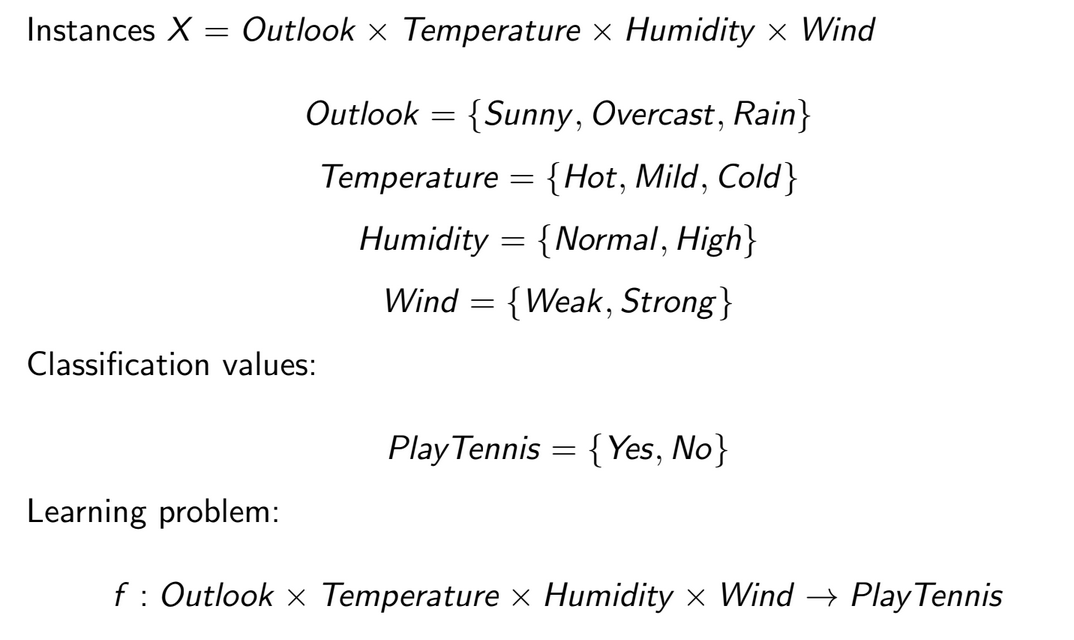
\includegraphics[width=12cm]{images/Decision Trees/Screenshot_20221004_141401.png}
    \caption{}
    \label{fig:image2.1}
\end{figure}

\begin{figure}[H]
    \centering
    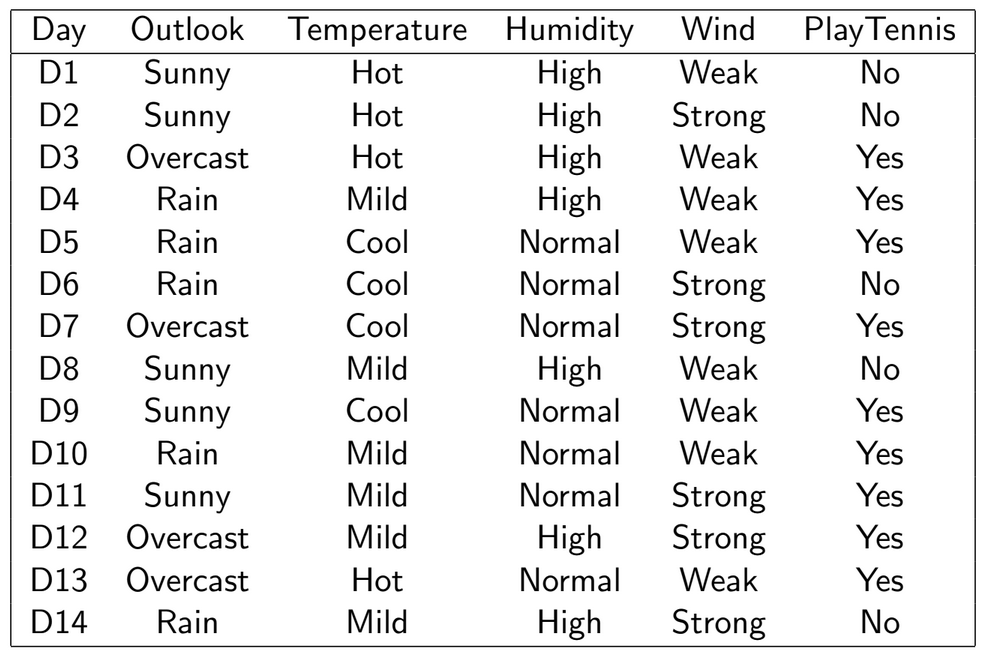
\includegraphics[width=12cm]{images/Decision Trees/Screenshot_20221004_141548.png}
    \caption{}
    \label{fig:image2.2}
\end{figure}


\begin{figure}[H]
    \centering
    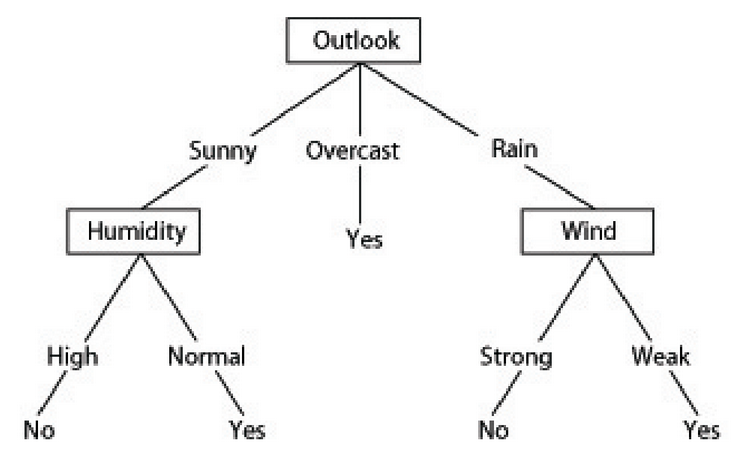
\includegraphics[width=12cm]{images/Decision Trees/Screenshot_20221004_141630.png}
    \caption{}
    \label{fig:image2.3}
\end{figure}

Decision trees represent a disjunction of conjunctions of constraints on the attribute values of instances.

\[(Outlook = Sunny \land Humidity = Normal)\] \[\lor\]
\[(Outlook = Overcast)\] \[\lor\]
\[(Outlook = Rain \land Wind = Weak)\]


\subsection{ID3 Algorithm}
Input: Examples, Target attribute, Attributes \\
Output: Decision Tree
\begin{enumerate}
    \item Create a Root node for the tree
    \item if all Examples are positive, then return the node Root with label +
    \item if all Examples are negative, then return the node Root with label -
    \item if Attributes is empty, then return the node Root with label = most common value of Target attribute in Examples
    \item Otherwise
    \begin{itemize}
        \item A $\xleftarrow[]{}$ the “best” decision attribute for Examples
        \item Assign A as decision attribute for Root
        \item For each value $v_{i}$ of A
         \begin{itemize}
             \item add a new branch from Root corresponding to the test A = $v_{i}$
             \item Examples$_{v_{i}}$ = subset of Examples that have value $v_{i}$ for A
             \item if Examples$_{v_{i}}$ is empty then add a leaf node with label = most common value of Target\_attribute in Examples
             \item else add the tree ID3(Examples$_{v_{i}}$ , Target\_{attribute}, Attributes-{A})
         \end{itemize}
    \end{itemize}
\end{enumerate}

Remember: Output tree depends on attribute order.

We have to measure which attribute gives us the best information

\subsubsection{Information Gain}
Information gain measures how well a given attribute separates the training examples according to their target classification. ID3 selects the attribute that induces highest information gain.

The Information Gain is measured as a reduction in entropy.

\begin{equation}
    Entropy(S) \equiv -p_{\oplus} \log_{2}p_{\oplus} - p_{\ominus} \log_{2}p_{\ominus}
\end{equation}

\begin{figure}[H]
    \centering
    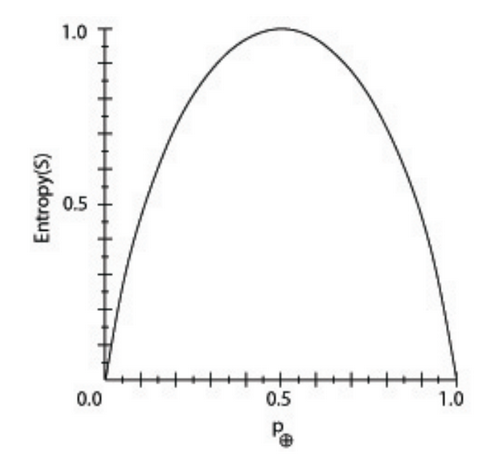
\includegraphics[width=12cm]{images/Decision Trees/Screenshot_20221004_143301.png}
    \caption{}
    \label{fig:image2.4}
\end{figure}

Consider the set S = [9+, 5-] (9 positive examples, 5 negative examples)

\[Entropy(s) = -(9/14)\log_{2}(9/14) -(5/14)\log_{2}(5/14) = 0.940\]


\begin{equation}
    Entropy(S) \equiv \sum_{i=1}^{c}-p_{i}\log_{2}p_{i}
\end{equation}

Now we can calculate the $Gain$, which is by definition the expected reduction in entropy fo S caused by knowing the value of an attribute A.
\begin{equation}
    Gain(S,A) \equiv Entropy(S) - \sum_{v \in Values(A)} \frac{|S_{v}|}{|S|}Entropy(S_v)
\end{equation}
where $Values(A)$ is the set of all possible values of A \\
$S_{v} = {s \in S | A(s) = v}$

\begin{figure}[H]
    \centering
    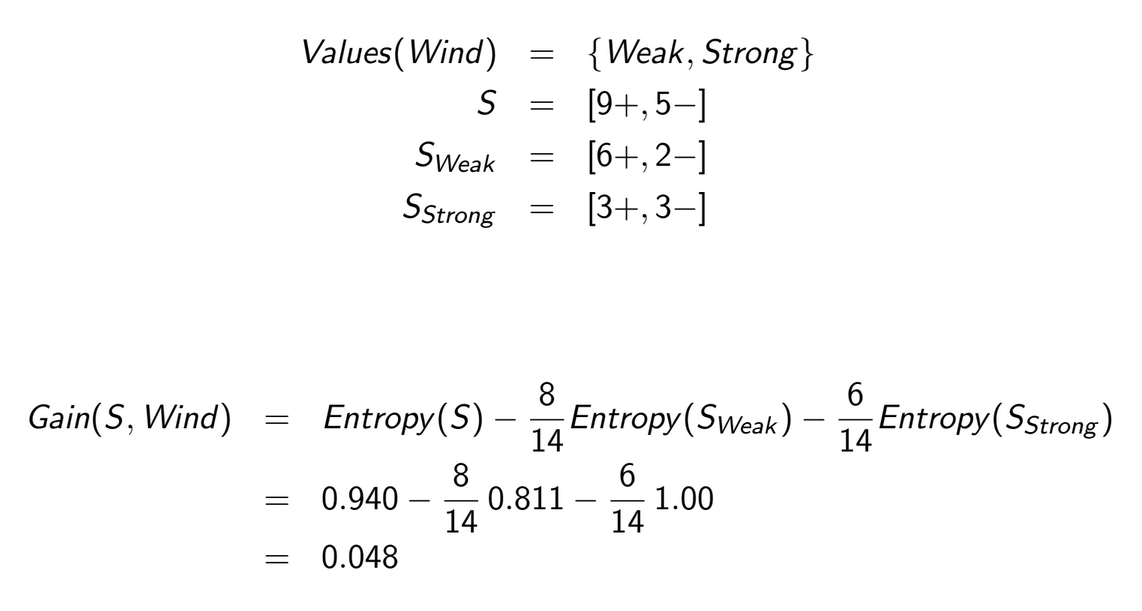
\includegraphics[width=12cm]{images/Decision Trees/Screenshot_20221004_144151.png}
    \caption{}
    \label{fig:image2.5}
\end{figure}

\begin{figure}[H]
    \centering
    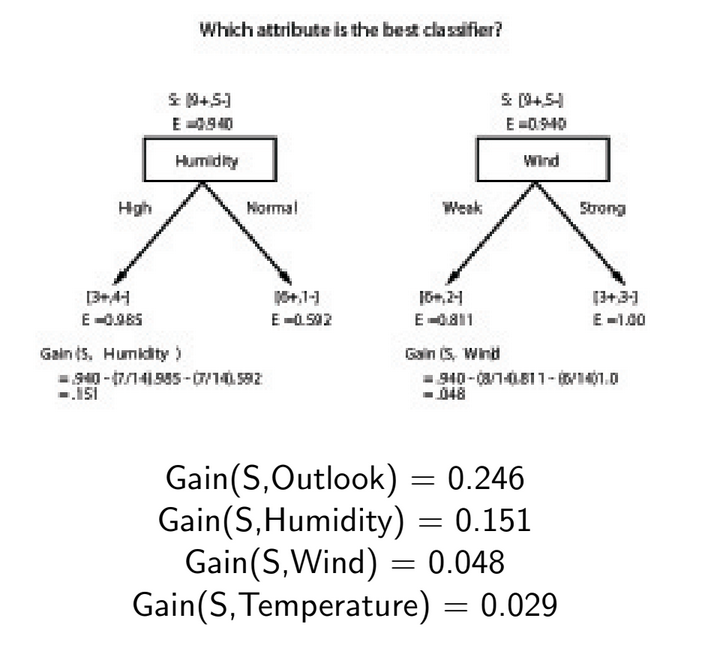
\includegraphics[width=12cm]{images/Decision Trees/Screenshot_20221004_144402.png}
    \caption{}
    \label{fig:image2.6}
\end{figure}

\subsection{Issues in Decision Tree Learning}
Determining how deeply to grow the DT \\
Handling continuous attributes \\
Choosing appropriate attribute selection measures \\
Handling training data with missing attribute values \\
Handling attributes with different costs \\

\vspace{0.5cm}

How can we avoid overfitting?
\begin{itemize}
    \item stop growing when data split not statistically significant
    \item grow full tree, then post-prune
\end{itemize}

To determine the correct tree size:
\begin{itemize}
    \item use a separate set of examples (distinct from the training examples) to evaluate the utility of post-pruning
    \item apply a statistical test to estimate accuracy of a tree on the entire data distribution
    \item using an explicit measure of the complexity for encoding the examples and the decision trees.
\end{itemize}

\subsubsection{Reduced-Error Pruning}

Split data into \emph{training} and \emph{validation} set \\
Do until further pruning is harmful (decreases accuracy):
\begin{itemize}
    \item Evaluate impact on validation set of pruning each possible node (remove all the subtree and assign the most common classification)
    \item Greedily remove the one that most improves validation set accuracy
\end{itemize}

By pruning the tree we are generating smaller and more accurate versions of the tree. Obviously, if the dataset is limited, pruning can led to bad result.

\subsubsection{Continuous variables}
 We can use discrete threshold and set rules based on them. As instance, if we have to measure the temperature, we can st a check "IF temperature > 30C$^{\circ}$"

\subsubsection{Attributes with many values}

We use the $GainRation$ instead

\begin{equation}
    GainRation(S,A) \equiv \frac{Gain(S,A)}{SplitInformation(S,A}
\end{equation}
\begin{equation}
    SplitInformation(S,A) \equiv - \sum_{i = 1}^{c}\frac{|S_{i}|}{|S|} \log_{2}\frac{|S_{i}|}{|S|}
\end{equation}
where $S_{i}$ is subset of S for which A has value $v_{i}$


\subsubsection{Attributes with Cost}

What if Attributes have costs related to them?

we can replace the gain with:
\begin{itemize}
    \item Tan and Schlimmer (1990)
    \begin{equation}
        \frac{Gain^{2}(S,A)}{Cost(A)}
    \end{equation}
    \item Nunez (1988) (w $\in$ [0, 1] determines importance of cost)
    \begin{equation}
        \frac{2^{Gain(S,A)} - 1}{(Cost(A) + 1)^{w}}
    \end{equation}
\end{itemize}

\subsubsection{Unknown Attribute values}

We can use training example anyway, sort through tree
\begin{itemize}
    \item If node n tests A, assign most common value of A among other examples sorted to node n
    \item assign most common value of A among other examples with same target value
    \item assign probability $p_{i}$ to each possible value $v_{i}$ of A
    \begin{itemize}
        \item assign fraction $p_{i}$ of example to each descendant in tree
    \end{itemize}
\end{itemize}

Classify new examples in same fashion

\subsection{Other algorithms based on Decision Trees}
Random Forests: this algorithm generates a collection of decision trees with some random criteria and integrates their values into a final result.

The Random criteria can be: 1) random subsets of data (bagging), 2) random subset of attributes (feature selection) etc.

The Integration of results is made by looking at the majority vote

Random forests are less sensitive to overfitting



\chapter{Probabilities}
\section{Probability}
\subsection{}section{Uncertainty}
We want to predict and approximate Uncertainty. 

A pure logical approach may not be fully realistic. It can lead to conclusions that are too weak for decision making. It also leads to non-optimal decisions.

We want to have a representation of uncertainty with probabilities.

\subsection{Probability}
\textbf{Sample space}: $\Omega$ is the sample space (set of possibilities). $\omega \in \Omega$ is a sample point/possible world/atomic event/outcome of a random process...

\textbf{Probability space} (or model): is a function $P: \Omega \xrightarrow[]{} R$ such that:
\begin{itemize}
    \item $0 \leq P(\omega)\leq 1$
    \item $\sum_{\omega \in \Omega} P(\omega) = 1$
\end{itemize}

\subsection{Event}
An event A is any subset of $\Omega$. \\
Probability of an event A is a function assigning to A a value [0, 1]
\begin{equation}
    P(A) = \sum_{\omega \in A} P(\omega)
\end{equation}
\subsection{Random Variables}
A \textbf{random variable} is a function from the sample space $\Omega$ to some range $X: \Omega \xrightarrow[]{}B$ \\
Example: $Odd: \Omega \xrightarrow[]{} Boolean$ \\
P introduces a probability distribution for a random variable X:
\begin{equation}
    P(X = x_{i}) = \sum_{\{\omega \in \Omega | X(\omega) = x_{i}\}} P(\omega)
\end{equation}
\subsection{Proposition}
A \textbf{proposition} is the event where an assignment to a random variable holds. Propositions can be combined using standard logical operators.
We can map functions to propositional logic.
\subsection{Syntax for proportions}
Propositional or Boolean random variables, Discrete random variables, Continuous random variables, Arbitrary Boolean combinations of basic proposition.
\subsection{Prior}
\textbf{Prior} or \textbf{unconditional} probabilities of propositions correspond to belief prior to arrival of any (new) evidence

\subsection{Probability Distribution}
A \textbf{probability distribution} is a function that assigns to each possible value of the random variable an apriori probability. The sum of all the values must be 1. Concepts of Probability distribution can be extended to continuous variables.

\subsection{Joint probability distribution}
\textbf{Joint probability distribution} for a set of random variables gives the probability of every atomic joint event of those random variables.

Joint probability distribution of two random variables is a grid where each cell is the sum of the probabilities of the event that correspond to the column and row.

\subsection{Conditional/Posterior probability}
Belief after the arrival of some evidence. I know the outcome of a random variable, how does this affect probability of other random variables?\\
$P(X=true|W=true) = ?$ \\
$P(X=true|W=true) \neq P(X=true, W=true) \neq P(X=true)$ \\
\subsubsection{Definition of conditional probability}
Conditional probability:
\begin{equation}
    P(a|b) \equiv \frac{P(a \land b)}{P(b)}\ if\ P(b) \neq 0
\end{equation}
Product rule:
\begin{equation}
    P(a \lor b) = P(a|b)P(b) = P(b|a)P(a)
\end{equation}
A general version holds for whole distributions.
\subsection{Total probabilities}

\begin{equation}
    P(a) = P(a|b)P(b) + P(a|\neg b)P(\neg b)
\end{equation}
in general, for a random variable Y accepting mutual exclusive values y:
\begin{equation}
    P(X) = \sum_{y_{i} \in D(Y)} P(X|Y=y_{i})P(Y=y_{i})
\end{equation}
D(Y): set of values for variable Y.

\subsection{Chain Rule}
\textbf{Chain rule} of derived by successive application of product rule:
\begin{equation}
    P(X_{1}, X_{2} = P(X_{1})P(X_{2}|X_{1}) \\
    P(X_{1} \dots X_{n}) = \prod_{i=1}^{n}P(X_{i}|X_{1}\dots X_{i-1})
\end{equation}

\subsection{Inference by enumeration}
\begin{figure}[H]
    \centering
    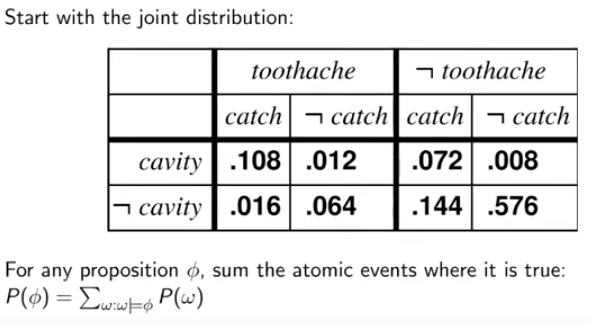
\includegraphics[width=12cm]{images/Probabilities/Inference_by_enum.png}
    \caption{}
    \label{fig:infbyenum}
\end{figure}

\subsection{Independence}
A and B are independent iff
$P(A|B) = P(A)$ or $P(B|A) = P(B)$ or $P(A, B) = P(A)P(B)$

Absolute independence is impossible.

\subsection{Conditional independence}

X is conditional independent from Y given Z iff $P(X|Y,Z) = P(X|Z)$ \\
$P(X,Y|Z) = P(X|Y,Z)P(Y|Z) = P(X|Z)P(Y|Z)$ \\

$Y_{i}$ conditional independent from $Y_{j}$ given Z:
\[P(Y_{1}\dots Y_{n}|Z) = P(Y_{1}|Z)\dots P(Y_{j}|Z)\]

Chain rule + conditional independence:
\[P(X,Y,Z) = P(X|Y,Z)P(Y,Z) = P(X|Y,Z)P(Y|Z)P(Z) = P(X|Z)P(Y|Z)P(Z)\]
\subsection{Bayes' Rule}
Product rule:
\[P(a\land b) = P(a|b)P(b) = P(b|a)P(b) = P(b|a)P(a) = \]
\[= Bayes'rule P(a|b) = \frac{P(b|a)P(a)}{P(b)}\]

\subsection{Bayesian networks}

Graphical notation for conditional independence assertions and hence for compact specification of full joint distributions.\\
Syntax:
\begin{enumerate}
    \item a set of nodes, one per variable
    \item a direct, acyclic graph
    \item a conditional distribution for each node given its parents 
\end{enumerate}
represented as a conditional probability table (CPT) giving the distribution over $X_{i}$ for each combination of parent values


\chapter{Bayesian Learning}
\section{Bayesian Learning}

\subsection{the problem}
We want to learn a function given a dataset D. We want the function to approximate a new given instance x' as close as possible to the real value.
\[v* = \underset{h \in H}{argmax} P(v|x', D)\]

Given a dataset D and hypothesis H, compute a probability distribution over H given D.
\[P(H|D)\]
we can apply Bayes rule
\[P(h|D) = \frac{P(D|h)P(h)}{P(D)}\]

\subsection{MAP Hypothesis}
\[P(h|D) = \frac {P(H|h)P(h)}{P(D)}\]
Generally we want the most probable hypothesis h given D.\\
Maximum A Posteriori hypothesis $h_{MAP}$:
\[h_{MAP} = \underset{h \in H}{argmax}P(h|D) = \underset{h \in H}{argmax} \frac{P(D|h)P(h)}{P(D)} = \underset{h \in H}{argmax} P(D|h)P(h)\]
We removed P(D) because it is constant and does not influence the argmax. \\
We don't always have information about the prior $P(h)$. We need a new definition.
\subsubsection{ML Hypothesis}
\[P(h|D) = \frac{P(D|h)P(h)}{P(D)}\]
If i assume $P(h_{i}) = P(h_{j})$, we can further simplify, and choose the Maximum Likelihood hypothesis:
\[h_{ML} = \underset{h \in H}{argmax} P(D|h)\]
And consider all the posterior with the same probability.

\subsection{Bruteforce MAP Hypothesis Learner}
Calculate the posterior probability for each hypothesis  and return the highest one.
\subsection{Bayes Optimal Classifier}
consider the target function $f:X \xrightarrow[]{}V, V = \{v_{1}\dots v_{k}\}$, data set D and a new instance x $ \not\in $ D:
\[P(v_{j}|x, D) = \sum_{h_{j} \in H} P(v_{j}|x, h_{i})P(h_{i}|D)\]
total probability over H. \\
$h_{j}$ does not depend  on $x \not\in D \xleftarrow[]{}P(h_{i}|x,D) = P(h_{i},D)$

\subsubsection{Bayes optimal classifier}
If we use MAP or ML, we only get the most probable hypothesis and it is not true that the most probable hypothesis is also the correct class given a sample x. We can make a step further and use Bayes Optimal Classifier to get the most probable class. Given a Bayes Optimal Classifier, we can predict the class $v_{j}$ of a new instance x as:
\[v_{OB} = \underset{v_{j} \in V}{arg max}\sum_{h_{i} \in H}P(v_{j}|x, h_{i})P(h_{i}|D)\]
As we can see, the classifier needs the conditional probability of the class given a sample and an hypothesis $i$, and the conditional probability of the hypothesis given the Dataset.

\subsection{General Approach}
Given dataset D with $d_{j} = \{0,1\}$ assuming a probability distribution $P(d_{j}|\Theta$ \\
Maximum likelihood estimation
\[\Theta _{ML} = \underset{\Theta}{argmax}\log P(d_{i}|\Theta).\]
We can apply this method to different distributions.

\subsubsection{Bayes Naive classifier}
We could consider each attribute of x $= \{sx_{1}, \dots, x_{n}\}$ as independent and use a Naive Bayesian Classifier to learn the probability of a given class:
\begin{equation}
    C_{NB} = \underset{argmax}{c_{j}} P(c_{j}|D) \prod_{i=0}^{n} P(x_{i}|c_{j}, D)
\end{equation}

The assumption is fundamental in Naive Bayes. However it is not true in the vast majority of real life situations. Still it behaves well. It is good for spam detection and document classification.


\chapter{Models For Classification}
\section{Probabilistic Models}
Assuming $P(C_{1}) = \pi$, $P(x|C_{i})\nu (x; \N _{i}, \Sigma$). Given the dataset $D = {(x_{n}, t_{n})^{N}_{n=1}}, t_{n}=1$ if $x_{n}$ belongs to class $C_{1}$, $T_{n} = 0$ otherwise.

$N_{1}$ is the number of samples in D belonging to $C_{1}$ and $N_{2}$ be the number of samples from $C_{2}$ ($N = N_{1} + N_{2}$).

The likelihood function is:
\begin{equation}
    P(t|\pi, \mu _{1}, \mu_{2}, \Sigma, D) = \prod_{n=1}^{N}[\pi \N (x_{n};\mu_{1}, \Sigma)]^{t_{n}}
    [(1 - \pi) \N (x_{n};\mu_{2}, \Sigma)]^{(1 - t_{n})}
\end{equation}
Determine $\pi, \mu_{!}, \mu_{2}, \Sigma$

By maximizing the log likelihood function we obtain:
\begin{equation}
    \pi = \frac{N_{1}}{N}, \\
    \mu_{1} = \frac{1}{N_{1}} \sum_{n=1}^{N}t_{n}x_{n}, \\
    \mu_{2} = \frac{1}{N_{2}} \sum_{n=1}^{N}t_{n}x_{n}, \\
    \Sigma = \frac{N_1}{N}S_{1} + \frac{N_2}{N}S_{2}. 
\end{equation}
with $S_{i} = \frac{1}{N_{i}} \sum_{n \in C_{i}}(x_{n} - \mu_{i})(x_{n} - \mu_{i})^{T}$, $i = 1, 2$.

If we want to predict a new sample $x'$:
\begin{equation}
    P(C_{1}|x') = \sigma (w^{T}x' + W_{0})
\end{equation}
\subsection{Multiple classes}

\begin{equation}
    P(C_{k}|x) = \frac{P(x|C_{k})P(C_{k})}{\sum_{j}P(x|C_{j})P(C_{j})} = \frac{exp(a_{k})}{\sum_{j}exp(a_{j})}
\end{equation}
with $a_{k} = \ln P(x|C_{k})P(C_{k})$\ \

\subsection{Gaussian Naive Bayes}
$P(C_{k}) = \pi_{k}, P(x|C_{k}) = \N(x: \mu_{k}, \Sigma)$
Data set $D = \{(x_{n}, t_{n})^{N}_{n=1}\}$, with $t_{n}$ 1-of-K encoding
\begin{equation}
    \pi = \frac{N_{k}}{N}, \\
    \mu_{k} = \frac{1}{N_{k}} \sum_{n=1}^{N}t_{nk}x_{n}, \\
    \Sigma = \sum_{k=1}^{K}\frac{N_k}{N}S_{k}, 
    S_{k} = \frac{1}{N_{k}} \sum_{n = 1}^{N} t_{nk}(x_{n} - \mu_{k})(x_{n} - \mu_{k})^{T}
\end{equation}
Prediction of new sample $x \not\in D$
\begin{equation}
    \underset{C_{k} \in C}{argmax} P(C_{k}|x) = \underset{k}{argmax}\frac{exp(a_{k})}{\sum_{j}exp(a_{j})}
\end{equation}
with $a_{k} = \ln P(x|C_{k}) P(C_{k})$

\subsection{Compact Notation}
Model:
\begin{equation}
    w^{T}x + w_{0} = (w_{0} w)(
    \begin{bmatrix} 
        1 \\
        x
    \end{bmatrix})
\end{equation}

\section{Discriminative models}
In the discriminative models we only want to compute the posterior probabilities without estimating the distribution. We can not sample new elements from the distribution

The likelihood for a parametric model $M_{\Theta}: P(t|\Theta, D), D = $ and the maximum likelihood solution is:
\begin{equation}
    \Theta^{*} = \underset{\Theta}{argmax}\ln P(t|\Theta, X)
\end{equation}
when $M _\Theta$ belongs to the exponential family, likelihood $P(t|\Theta, X)$ can be expressed in the form $P(t|\Tilde{w}, X)$, with maximum likelihood
\begin{equation}
    \Tilde{w}^{*} = \underset{\Tilde{w}}{argmax} ln P(t|\Tilde{w}, X)
\end{equation}
Without estimating the model parameters. Simplified notation: $P(t|\Tilde{w})$

\subsection{Logistic regression}
\subsubsection{Two classes}
given the dataset $D$ with each sample of the dataset $t_{i} \in \{0, 1\}$

Likelihood function:
\begin{equation}
    p(t|\Tilde{w}) = \prod_{n=1}^{n} y^{t_{n}}_{n}(1 - y_{n})^{1 - t_{n}}
\end{equation}
with 
\[t_{n} = p(C_{1}|\Tilde{x}_{n}) = \sigma(\Tilde{w}^{T}\Tilde{x}_{n}) = \frac{1}{1 + e^{-\Tilde{w}^{T}\Tilde{x}_{n}}}\]

If we use the logarithm of the previous formula as loss function, we get the cross entropy error function (negative log likelihood)
\begin{equation}
    E(\Tilde{w}) \equiv -\ln P(t|\Tilde{w}) = -\sum^{N}_{n=1} [t_{n}\ln y_{n} + (1 - t_{n}) \ln (1 - y_{n})]
\end{equation}

We have to solve $\Tilde{w}^{*} = \underset{\Tilde{w}}{argmin}E(\Tilde{w})$. Many solvers are available for this problem.

\paragraph{Iterative reweight least squares}
Neqton-Raphson iterative optimization for minimizing the Gradient of the error wrt $\Tilde{w}$
\begin{equation}
    \nabla E(\Tilde{w}) = \sum_{n=1}^{N}(y_{n} - t_{n})\Tilde{x}_{n}
\end{equation}
Gradient descent step
\begin{equation}
    \Tilde{w} \xrightarrow[]{} \Tilde{w} - H(\Tilde{w})^{-1}\nabla E(\Tilde{w})
\end{equation}
where $H(\Tilde{w}) = \nabla \nabla E(\Tilde{w})$ is the Heissan matrix of $E(\Tilde{w})$

Classify a new sample $\Tilde{x}'$ as $C_{k}$ where $k^{*} = \underset{k=1\dots K}{argmax} P(C_{k}|\Tilde{x}', \Tilde{w}^{*})$

\paragraph{Generalization}
if we have a target function $f: X \xleftarrow{}C$ and a dataset $D$ we define an error function $E(\Theta)$ and solve the optimization problem
\begin{equation}
    \Theta^{*} = \underset{\Theta}{argmin} E(\Theta)
\end{equation}
and classify a new sample as $y(x'; \Theta^{*})$

\subsubsection{Learning in feature space}
we can replace $x_{n}$ with $\Phi(x_{n})$ to transform the dataset in an input space to get $\Phi'$ (we transform the dataset).

\paragraph{Compact notion}
two classes:
\begin{equation}
    y(x) = w^{T}x + w_{0} = \Tilde{w}^{T}\Tilde{x}
\end{equation}
with
\begin{equation}
    \Tilde{w} = \begin{bmatrix} 
                    w_{0} \\
                    w
                \end{bmatrix},
    \Tilde{x} = \begin{bmatrix} 
                    1 \\
                    x
                \end{bmatrix}
\end{equation}
with k classes there are more rows

\paragraph{Multiple classes}
Cannot use combination of binary linear models!!!
One-versus-the-rest classifiers and one-versus-one-classifiers. We can instead use K-class discriminant comprising K linear functions. Then classify x as $C_{k}$ if $y_{k}(x) > y_{j}(x)$ for all $j \neq k$. Decision boundary between $C_{k}$ and $C_{j}$:
\begin{equation}
    (\Tilde{w}_{k} - \Tilde{w}_{j})^{T}\Tilde{x} = 0
\end{equation}

\section{Learning linear discriminant}
methods to solve the linear discriminant problem
\subsection{Least Squares}
Given the dataset $D$, use 1 of K coding scheme, where each row is $t_{n} = (0, \dots, 1, \dots, 0)^{T}$

Minimize
\begin{equation}
    E(\Tilde{W}) = \frac{1}{2} \Tr{(\Tilde{X}\Tilde{W}\ T)^{T} ( \Tilde{X}\Tilde{W}\ T)}
\end{equation}
where:
\begin{equation}
    \Tilde{W} = (\Tilde{X}^T\Tilde{X})^{-1}(\Tilde{X}^{T}\ T)
\end{equation}
the $(\Tilde{X}^T\Tilde{X})^{-1}$ term is usually called pseudo inverse and is denoted as $X^{\dagger}$. Note: Least square is not robust to outliers.

\subsection{Perceptron}

\begin{figure}[H]
    \centering
    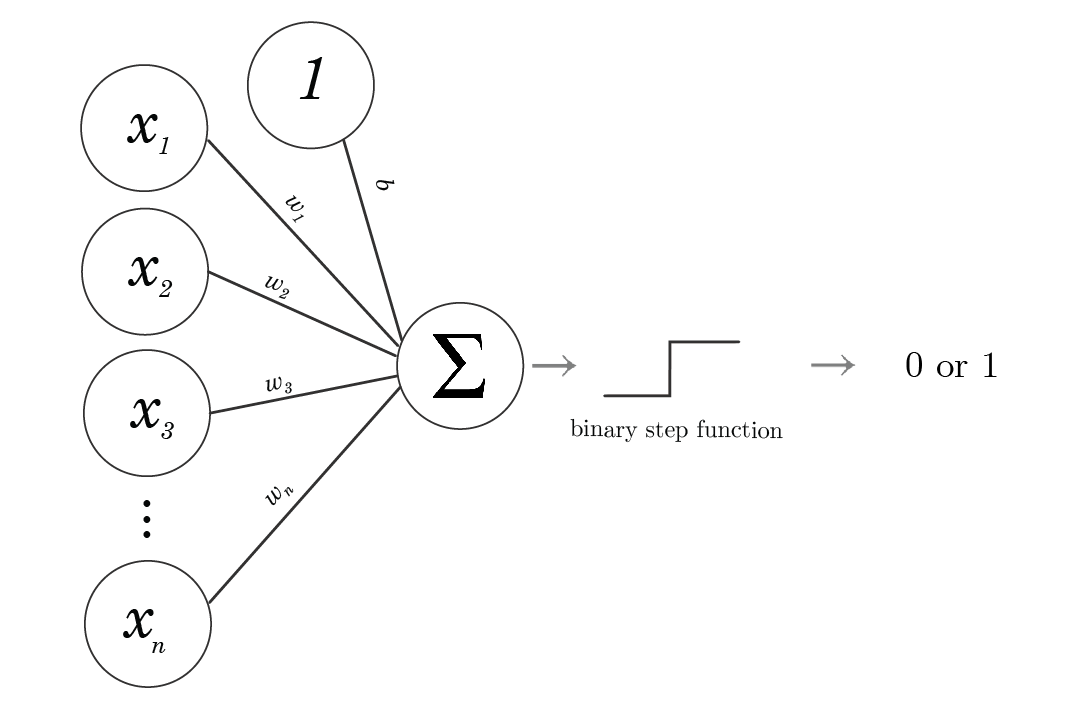
\includegraphics[width=15cm]{images/Probabilistic Models/perceptron.png}
    \caption{}
    \label{fig:perceptron}
\end{figure}

$o(x_{1}, \dots, x_{d})$ is 1 if $w_{0} + w_{1}x_{1} + \dots +w_{0} + w_{n}x_{n} > 0$, -1 otherwise.

The perceptron training rule is to minimize the squared error (loss function):
\begin{equation}
    E(w) \equiv \frac{1}{2}\sum_{n=1}^{N}(t_{n} - o_{n})^{2} = \frac{1}{2} \sum_{n=1}^{N}
(t_{n} - w^{T}x_{n})^2\end{equation}

if we calculate the derivative of the error function we get:
\begin{equation}
    \frac{\partial E}{\partial w_{i}} = \dots = \sum_{n=1}^{N}(t_{n} - w^{T}x_{n})(-x_{i,n})
\end{equation}

and then we use this derivative to move weights towards the the minimum.
\begin{equation}
    w_{i} \xleftarrow{} w_{i} + \eta \Delta w_{i}
\end{equation}
where $\Delta w_{i}$ is the derivative of the loss. 

Perceptron converge if training data is clearly separable and the learning rate $\eta$ is sufficiently small.
It can terminate if the error reaches a threshold or there is a max number of iterations.

\subsection{Ficher's linear discriminant}
adjust w to find a direction that maximizes class separation based on the projection on the line. Consider a data set with $N_{1}$ points in $C_{1}$ and $N_{2}$ points in $C_{2}$
\begin{equation}
    m1 = \frac{1}{N_{1}}\sum_{n \in C_{1}}x_{n}
\end{equation}
\begin{equation}
    m2 = \frac{1}{N_{2}}\sum_{n \in C_{2}}x_{n}
\end{equation}
choose w that maximizes $J(w) = w^{t}(m_{2} - m_{1})$, subject to $||w|| = 1$
\begin{equation}
    w \propto S^{-1}_{W}(m_{2} - m_{1})
\end{equation}

we have to maximize 
\begin{equation}
    J(w) = \frac{w^{T}S_{B}w}{w^{T}S_{W}w}
\end{equation}
by solving $\frac{d}{dw}J(w) = 0$. In this formula, $S_{B}$ is the between covariance matrix while $S_{w}$ is the within covariance matrix.

\subsection{Support Vector Machines}
Support Vector Machines (SVM) for classification aims at finding a maximizing the margin providing better accuracy.

Assume that the dataset is linearly separable,

let $x_{k}$ be the closest point of the data set $D$ to the hyperplane $\overline{h}: \overline{w}^{T}x + \overline{w_{0}}$.
The \textbf{margin} (smallest distance between $x_{k}$ and $\overline{h}$) is $\frac{y(x_{k}}{||w||}$
So, given a dataset, the margin is computed as: 
\begin{equation}
    \underset{n=1, \dots , N}{min} \frac{y(x_{k})}{||w||} = \dots = \frac{1}{||w||} \underset{n=1, \dots , N}{min} [t_{n}(\overline{w}^{T}x_{n} + \overline{w_{0}})]
\end{equation}
using the property $|y(x_{n})| = t_{n}y(x_{n})$

Now we can calculate the hyperplane with the maximum margin by maximizing:
\begin{equation}
    w^{*}, w_{0}^{*} = \underset{w, w_{0}}{argmax} \frac{1}{||w||} \underset{n=1, \dots , N}{min} [t_{n}(w^{T}x_{n} + w_{0})]
\end{equation}
We can rescale the dataset such that the closest point $x_{k}$ has:
\begin{equation}
    t_{k}(w^{T}x_{k} + w_{0}) = 1
\end{equation}
and each other point has margin $\geq 1$

When we find the maximum margin hyperplane $w^{*}, w_{0}^{*}$, there will be at least 2 closest points $x_{k}^{\oplus}$ and $x_{k}^{\ominus}$ (one for each class).
The margin for $x_{k}^{\oplus}$ will be +1 while the margin for $x_{k}^{\ominus}$ will be -1.

In order to find a solution to he problem:
\begin{equation}
    w^{*}, w_{0}^{*} = argmax \frac{1}{||w||} = argmin \frac{1}{2} ||w||^{2}
\end{equation}
subject to:
\begin{equation}
    t_{n}(w^{T}x_{n} + w_{0}) \geq 1 \forall n = 1, \dots, N
\end{equation}
we can use the quadratic programming solution with the Lagrangian method.
The solution will be:
\begin{equation}
    w^{*} = \sum_{n=1}^{N} a_{n}^{*}t_{n}x_{n}
\end{equation}
$a_{i}^{*}$ (Lagrange multipliers): result of the Lagrangian optimization problem:
\begin{equation}
    \Tilde{L}(a) = \sum_{n=1}^{N}a_{n} - \frac{1}{2} \sum_{n=1}^{N}\sum_{m=1}^{N}a_{n}a_{m}t_{n}t_{m}x_{n}^{T}x_{m}
\end{equation}
subject to
\begin{equation}
    \begin{multlined}
        a_{n} \geq 0 \ \forall n = 1, \dots, N \\
        \sum_{n=1}^{N}a_{n}t_{n} = 0
    \end{multlined}
\end{equation}

\paragraph{Notes}
samples $x_{n}$ for which $a_{n}^{*} = 0$ will not count to the solution. \\
Karush-Kuhn-Tucker (KKT) condition:
for each $x_{n} \in D$, either $a_{n}^{*} = 0$ or $t_{n}y(x_{n}) = 1$ \\
thus $t_{n}y(x_{n}) > 1$ implies $a_{n}^{*} = 0$ \\
Support vectors are those points such that $t_{k}y(x_{k}) = 1$ and $a_{k}^{*} > 0$
\begin{equation}
    SV \equiv \{x_{k} \in D | t_{k}y(x_{k}) = 1\}
\end{equation}

If we want to express the hyperplane with his support vectors we can use:
\begin{equation}
    y(x) = \sum_{x_{j} \in SV}a_{j}^{*}t_{j}x^{T}x_{j}\text{ è }w_{0}^{*} = 0
\end{equation}

To compute $w_{0}^{*}$, we have to find support vectors that satisfies $t_{k}y(x_{k}) = 1$:
\begin{equation}
    t_{k}(\sum_{x_{j} \in SV}a_{j}^{*}t_{j}x_{k}^{T}x_{j}) = 1
\end{equation}
multiplying by $t_{k}$ and using $t_{k}^{2} = 1$ 
\begin{equation}
    w_{0}^{*} = t_{k} - \sum_{x_{j} \in SV}a_{j}^{*}t_{j}x_{k}^{T}x_{j}
\end{equation}

Instead of using one particular support vector $x_{k}$ to determine $w_{0}$, a more stable solution can be obtained by averaging over all the support vectors:
\begin{equation}
    w_{0}^{*} = \frac{1}{|SV|}\sum_{x_{k} \in SV}\left(t_{k} - \sum_{x_{j} \in S} a_{j}^{*}t_{j}x_{k}^{T}x_{j}\right)
\end{equation}

In order to classify a new instance, we can look at the sign:
\begin{equation}
    y(x') = sign\left(\sum_{x_{k} \in SV} a_{j}^{*}t_{j}x'^{T}x_{j}\right)
\end{equation}

\paragraph{Soft margin}
If data is almost linearly separable, we can use a soft margin $\xi _{n} \geq 0,\ n=1, \dots, N$ (called slack variable).
A soft margin lets some of the points to lay between the support vectors, adding a border.
\begin{equation}
    \begin{multlined}
        t_{n}y(x_{n}) \geq 1 - \xi _{n}, \ n=[1, \dots, N] \\
        w^{*}, w_{0}^{*} = \argmin \frac{1}{2} ||w||^{2} + C\sum_{n=1}^{N}\xi_n{} \\
        subject\ to\\
        t_{n}y(x_{n}) \geq 1 - \xi_{n}, \ n=1, \dots, N\\
        \xi_{n} \geq 0, n=1, \dots, N
    \end{multlined}
\end{equation}
where $C$ is a constant.

\subsection{Basis Function}
Until now, we considered only models that work directly on the dataset $D$, but what if we first perform a non-linear transformation of the inputs $\Phi  (x)$ (basis function)?.\\
By transforming the data, we can then find a linear hyperplane for the feature space $\Phi (D)$ that is not linear in the original space of $D$, actually separating points that were not linearly separable before the transformation.


\begin{figure}[H]
    \centering
    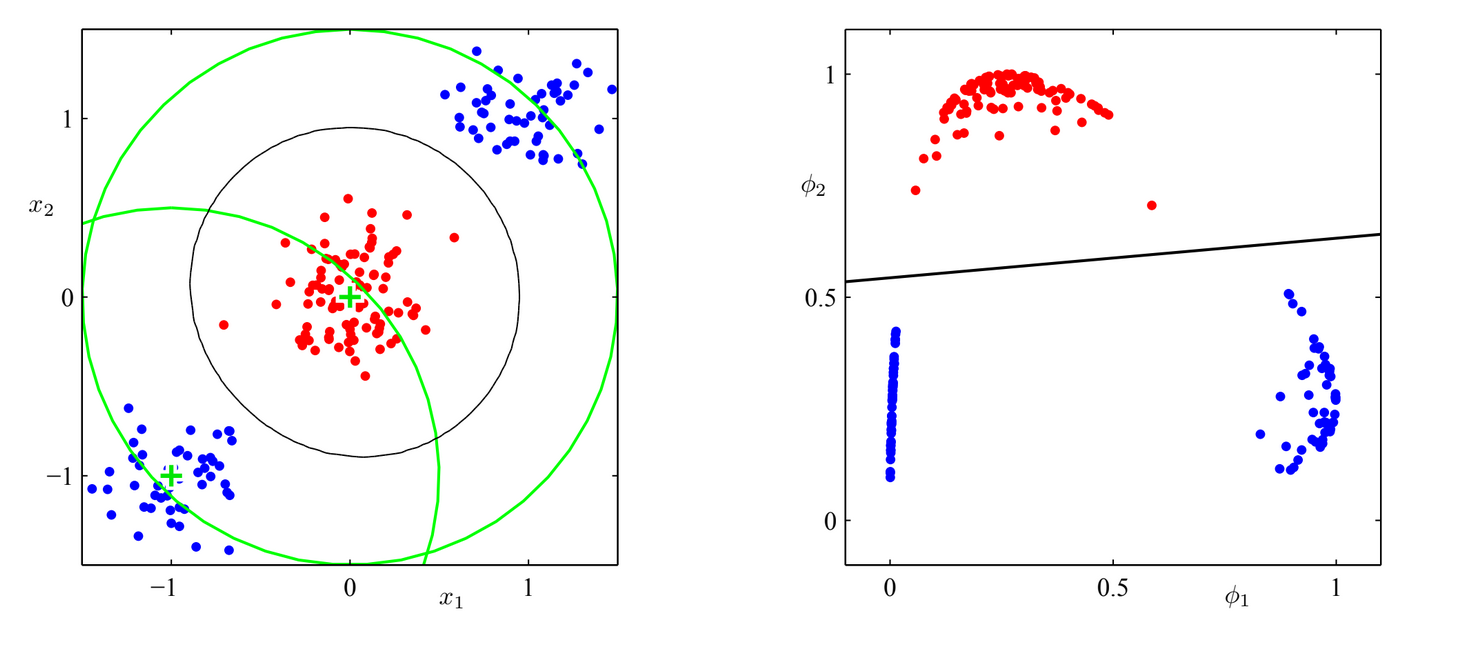
\includegraphics[width=15cm]{images/Probabilistic Models/phi_on_dataset.png}
    \caption{}
    \label{fig:phi_on_dataset}
\end{figure}

What we actually do is to train a linear model on a non-linear transformation:
\begin{equation}
    \begin{multlined}
    y(x) = w^{T}\phi(x) + w_{0} \text{    (two classes)} \\
    y_{k}(x) = w_{k}^{T}\phi(x) + w_{k0}\text{    (multiple\ classes)} \\
    \end{multlined}
\end{equation}


\chapter{Linear Regression}
\section{Linear Models for Regression}
\subsection{What we want to do?}
We have a dataset $d = \{(x_{n}, t_{n})_{n=1}^{N}\}$ and we want to learn a function $f: X \xrightarrow[]{}Y$ with $X \subseteq \mathcal{R}^{d}$ and $Y = \mathcal{R}$ \\
The model is such that $y(x; W) = W^{T}x$ approximates the target function ($W$ are weights of the function).

Linear model for linear functions
\begin{equation}
    y(x;w) = w_{0} + w_{1}x_{1} + \dots + w_{d}x_{d} = w^{T}x
\end{equation}
with $x = \begin{bmatrix} 1\\ x_{1} \\ \dots \\ x_{d} \\ \end{bmatrix}$ and $w = \begin{bmatrix} w_{0}\\ w_{1} \\ \dots \\ w_{d} \\ \end{bmatrix}$\\
Using non-linear functions of input variables means having:
\begin{equation}
    y(x;w) = \sum_{j=0}^{M}w_{j}\phi_{j}(x) = w^{T}\phi(x)
\end{equation}
with $w = \begin{bmatrix} w_{0}\\ w_{1} \\ \dots \\ w_{d} \\ \end{bmatrix}$,  $x = \begin{bmatrix} \phi_{0}(x)\\ \phi_{1}(x) \\ \dots \\ \phi_{M}(x) \\ \end{bmatrix}$ and $\phi_{0}(x) = 1$ (still linear in the parameter $w$).

\subsection{Example of basis function}
We can define a set of functions:
\begin{equation}
    \Phi(x) = \begin{bmatrix}
                \phi_{0}(x)\\
                \dots \\
                \phi_{M}(x)
                \end{bmatrix}
\end{equation}
such that $y(x;W) = W^{T}\Phi(x)$ is linear in $W$ and not linear in $x$.

Well known transformations are for example:
\begin{equation}
    \Phi(x) = \begin{bmatrix}
                1\\
                x \\
                x^{2} \\
                x^{3} \\
                \dots \\
                x^{M} \\
                \end{bmatrix}
\end{equation}
Other used transformations are Radial, Sigmoid and Tanh

\subsection{maximum Likelihood and least square}

Target value t is given by the model $y(x; w)$ affected by additive noise $\epsilon$: $t = y(x;w) + \epsilon$\\
Assume Gaussian noise $P(\epsilon|\beta) = \N(\epsilon|0, \beta ^{-1})$, with precision $\beta$. We have:
\begin{equation}
    P(t|x,w,\beta) = \N(t|y(x;w),\beta ^{-1})
\end{equation}

If we get all the labels $t_{n}$, regroup them in a single vector $t$ and assume they are all independent, we can seek the maximum likelihood function:
\begin{equation}
    p(t|x_{1}, \dots, x_{N}, w, \beta) = \prod_{n=1}^{N}\N(t_{n}|w^{T}\phi(x_{n}), \beta^{-1})
\end{equation}
or equivalently, we can consider the natural logarithm:
\begin{equation}
    \begin{multlined}
    \ln p(t|x_{1}, \dots, x_{N}, w, \beta) = \sum_{n=1}^{N}\ln \N(t_{n}|w^{T}\phi(x_{n}), \beta^{-1}) = \\
    \frac{N}{2} \ln (\beta) - \frac{N}{2}\ln (2\pi) - \beta E_{D}(w)
    \end{multlined}
\end{equation}
where we use the sum-of-squares error function.
\begin{equation}
    argmin\ E_{D}(w) = argmin\ \frac{1}{2}\sum_{n=1}^{N}[t_{n} - w^{T}\phi(x_{n})]^{2}
\end{equation}
The gradient of the function is then:
\begin{equation}
    \nabla \ln p(t|w, \beta) = \beta \sum_{n = 1} ^{N} \{t_{n} - w^{T}\phi(x_{n})\} \phi(x_{n})^{T}
\end{equation}
We can solve the problem in two ways:
\begin{enumerate}
    \item \textbf{Close Form Solution} 
        if we set the gradient of $E_{D}(w)$to zero and solve for w we obtain:
        \begin{equation}
            w_{ML} = (\Phi^{T}\Phi)^{-1}\Phi^{T}t
        \end{equation}
        where t is the array $t = \begin{bmatrix} t_{0}\\ w_{1} \\ \dots \\ t_{dN} \\ \end{bmatrix}$ and $\Phi$ is
        $\Phi = \begin{bmatrix} \phi_{0}(x_{1}) & \dots & \phi_{M}(x_{1}) \\ \phi_{0}(x_{2}) & \dots & \phi_{M}(x_{2}) \\ \dots & \dots & \dots \\ \phi_{0}(x_{N}) & \dots & \phi_{M}(x_{N})) \end{bmatrix}$.

        Notice: $(\Phi^{T}\Phi)^{-1}\Phi^{T}$ is the \textit{pseudo-inverse} $\Phi^{\dagger}$
    \item \textbf{Iterative Solution}: this method does not deliver the optimal solution, but a good enough one (Close Form Solution might be too much costly in term of computation). \\
    Stochastic Gradient Descent algorithm:
    \begin{equation}
        \hat{w} \xleftarrow{} \hat{w} - \eta\nabla E_{n}
    \end{equation}
    therefore:
    \begin{equation}
        \hat{w} \xleftarrow{} \hat{w} - \eta[t_{n} - \hat{w}^{T}\phi(x_{n})]\phi(x_{n})
    \end{equation}
\end{enumerate}

None of these methods can actually solve the method.

\subsubsection{Regularization}
For Stochastic gradient descent, regularization is crucial. We have to choose the right $\eta$ in order to avoid overfitting.
One of the simplest regularizer is given by the sum-of-squares of the weight vector elements. 

If we consider:
\begin{equation}
    E_{D}(w) + \lambda E_{W}(w)
\end{equation}
where $\lambda$ is the regularizer that control the relative importance of the data-dependent error $E_{D}(w)$ and the regularization term $E_{W}(w)$. The sum-of-squares is:
\begin{equation}
    E_{W}(w) = \frac{1}{2} w^{T}w
\end{equation}
Another common function is:
\begin{equation}
    E_{W}(w) = \sum_{j=0}^{M}|w_{j}|^{q}
\end{equation}
This technique is also known as \textit{weight decay} since it penalizes the weights and tents to lower them towards zero, unless supported by the data.

\subsubsection{Multiple Outputs}
We can introduce a different set of basis functions for each component of $t$, leading to multiple, independent regression problems. another interesting method is using the same set of basis functions to model all of the components of the target vectors so that
\begin{equation}
    t(x, w) = W^{T}\phi(x)
\end{equation}
where y is a K-dimensional column vector, $W$ is a $M \times K$ matrix of parameters, and $\phi(x)$ is a $M$-dimensional column vector with elements $\phi_{j}(x)$ and $\phi_{0}(x) = 1$.

We can combine a set of observations $t_{1}, \dots, t_{N}$ into a matrix $T$ of size $N \times K$ such that the $n^{th}$ row is given by $t_{n}^{T}$. Similarly, we can combine the input vectors $x_{1}, \dots, x_{N}$ into a matrix X. The log likelihood is then:
\begin{equation}
    \ln p(T|X, W, \beta) = \sum_{n=1}^{N}\ln \N(t_{n}|W^{T}\phi(x_{n}), \beta^{-1}I) = \\
    \frac{NK}{2} \ln (\frac{\beta}{2\pi}) - \frac{\beta}{2} \sum_{n=1}^{N} ||t_{n} - W^{T}\phi(x_{n})||^{2}
\end{equation}
As before, we can maximize the function wrt $W$:
\begin{equation}
    W_{ML} = (\Phi^{T}\Phi)^{-1}\Phi^{T}T
\end{equation}
where, for each target variable $t_{k}$, we have:
\begin{equation}
    w_{k} = (\Phi^{T}\Phi)^{-1}\Phi_{T}t_{k} = \Phi^{\dagger}t_{k}
\end{equation}

\chapter{Kernel Methods}
\section{Kernel Methods}

Some of the linear parametric models can be re-cast into an equivalent 'dual representation' in which the predictions are also based on linear combination of a kernel function evaluated at training time on training points.

\subsection{Approach}
We use a similarity measure $k(x, x') \geq 0$ between the instances $x, x'$. $k(x, x')$ is called kernel function.\\ 
If we have $\phi(x)$, a possible choice is $k(x, x') = \phi(x)^{T}\phi(x')$

\subsection{Kernel}
A kernel is a real-valued function $k(x, x') \in \mathcal{R}$ for $x, x' \in \mathcal{X}$, where $\mathcal{X}$ is some abstract space. A kernel typically satisfies the following conditions:
\begin{enumerate}
    \item symmetric: $k(x, x') = k(x', x)$
    \item non-negative: $k(x, x') \geq 0$
\end{enumerate}
(not strictly required)

\subsubsection{Input normalization}
Input dataset $D$ must be normalized in order for the kernel to be a good similarity measure in practice. If we don't do that, the solution may be affected.\\
Types of normalization:
\begin{itemize}
    \item min-max:      $\overline{x} = \frac{x - min}{max - min}$
    \item normalizaiton:        $\overline{x} = \frac{x - \mu}{\sigma}$
    \item unit vector:      $\overline{x} = \frac{x}{||x||}$
\end{itemize}

Kernel families:
\begin{itemize}
    \item \textbf{Linear}: $k(x, x') = x^{T}x'$
    \item \textbf{Polynomial}: $k(x, x') = (\beta x^{T}x' + \gamma)^{d}, \ d \in \{2,3,\dots\}$
    \item \textbf{Radial Basis Function (RBF)}: $k(x, x') = exp(- \beta | x - x'|^{2})$
    \item \textbf{Sigmoid}: $k(x, x') = tanh(\beta x^{T}x' + \gamma)$
\end{itemize}

\subsection{How do we use the kernels?}
Consider a linear model $y(x; w) = w^{T}x$ with a dataset $D$. \\
Minimize $J(w) = (t - Xw)^{T}(t - Xw) + \lambda ||w||^{2}$\\
$X = \begin{bmatrix} x_{1}^{T} \\ \dots \\ x_{N}^{T} \end{bmatrix}$ design matrix, $t = \begin{bmatrix} t_{1} \\ \dots \\ t_{N} \end{bmatrix}$ output vector.\\
The optimal solution is:
\begin{equation}
    \hat{w} = (X^{T}X + \lambda I_{N})^{-1}X^{T}t = X^{T}(XX^{T} + \lambda I_{N})^{-1} t
\end{equation}
with $I_{n}$ an $N \times N$ identity matrix.\\
We can call $\lambda = (XX^{T} + \lambda I_{N})^{-1} t$ and express our solution as:
\begin{equation}
    \hat{w} = X^{T}\alpha = \sum_{n=1}^{N} \alpha_{n}x_{n}
\end{equation}
which is a linear combination of coefficient $\alpha_{n}$\\
We can then write: $y(x; \hat{w} = \hat{w}^{T}x = \sum_{n=1}^{N} \alpha_{n} x_{n}^{T} x$. If we then consider a linear kernel $k(x, x') = x^{T}x'$, we can rewrite the model as
\begin{equation}
    y(x;\hat{w}) = \sum_{n=1}^{N} \alpha_{n} k(x_{n}, x)
\end{equation}
with $\alpha = (K + \lambda I_{N})^{-1}t$, and $K = XX^{T}$ is the \textbf{Gram Matrix}.

\subsubsection{Recap}
We can use the kernel $k(x,x') = x^{T}x'$ and express a model $y(x; \alpha)$ as the linear combination of $\alpha$ and $x_{n}^{T}X$, where $\alpha$ is the gram matrix summed to $\lambda I_{N}$, inverted and multiplied by $t$.\\
The \textbf{Gram matrix} is the dot product of all the possible points in the dataset.

\subsubsection{Trick of kernel}
We can use the same problem formulation and solution for every kernel, even if it is not linear.

Kernel trick or kernel substitution: If input vector $x$ appears in an algorithm only in the form of an inner
product $x^{T}x'$, replace the inner product with some kernel $k(x, x')$.

\subsubsection{SVM with kernel method}
In SVM, the solution has the form:
\begin{equation}
    w^{*} = \sum_{n=1}^{N} \alpha_{n}x_{n}
\end{equation}
the linear model with a linear kernel is:
\begin{equation}
    y(x; \alpha) = sign(w_{0} + \sum_{n=1}^{N} \alpha_{n} x_{n}^{T} x)
\end{equation}
and the kernel trick is:
\begin{equation}
    y(x; \alpha) = sign(w_{0} + \sum_{n=1}^{N} \alpha_{n} k(x_{n},x))
\end{equation}
Lagrangian problem for kernelized SVM classification
\begin{equation}
    \Tilde{L}(a) = \sum_{n=1}^{N}a_{n} - \frac{1}{2} \sum_{n=1}^{N}\sum_{m=1}^{N}a_{n}a_{m}t_{n}t_{m}k(x_{n},x_{m})
\end{equation}
solution:
\begin{equation}
    \begin{multlined}        
    a_{n} = \dots \\
    w_{0} = \frac{1}{|SV|} \sum_{x_{i} \in SV} (t_{i} - \sum_{x_{j} \in S} a_{j}t_{j}k(x_{i}, x_{j})
    \end{multlined}
\end{equation}
The main problem for kernelized methods is that we have to deal with a matrix that exponentially grows with the size of the dataset.
For most of the elements in SVM, the Lagrangian multiplier will be zero and so, only a subset of the values in the Gramm matrix are used for the solution, making the approach good for this case.
\subsubsection{Linear regression and kernels}
For linear regression the problem is that the computation of $K$ requires $> N^{2}$ operations and $K$ is not sparse, making the approach too costly for usage on big datasets.

What we can do for linear regression is instead use a different error function:
\begin{equation}
    E_{\epsilon}(y, t) = \{\begin{array}{lr}
        0, & \text{if } |y - t| < \epsilon\\
        |y - t| - \epsilon, & \text{otherwise}
        \end{array}
\end{equation}

\begin{figure}[H]
    \centering
    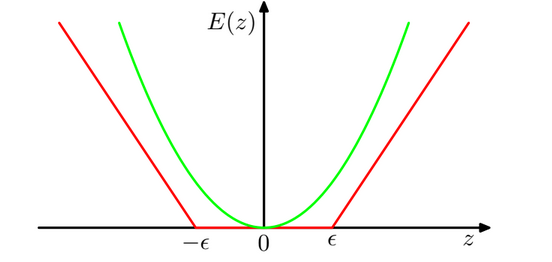
\includegraphics[width=15cm]{images/Kernel Methods/ksvm.png}
    \label{fig:ksvm}
    \caption{error function for linear regression that makes the kernel sparse.}
\end{figure}

Problem: it is not differentiable, so it is difficult to solve.

We can the introduce \textit{slack variables} $\xi_{n}^{+}, \xi_{n}^{-} \geq 0$:
\begin{equation}
\label{eq:ksvm_condition1}
    \begin{multlined}
        t_{n} \leq y_{n} + \epsilon + \xi_{n}^{+} \\
        t_{n} \leq y_{n} - \epsilon - \xi_{n}^{-}
    \end{multlined}
\end{equation}
Points that are into the $\epsilon$-tube $y_{n} - \epsilon \leq t_{n} \leq t_{n} + \epsilon \Rightarrow \xi_{n} = 0$
\begin{equation}
\label{eq:ksvm_condition2}
    \begin{multlined}
        \xi_{n}^{+} > 0 \Rightarrow y_{n} + \epsilon \\
        \xi_{n}^{-} > 0 \Rightarrow y_{n} - \epsilon
    \end{multlined}
\end{equation}
with $y_{n} = t(x_{n}, w)$. \\
The loss function can be rewritten as:
\begin{equation}
    J(w) = C\sum_{n=0}^{N}(\xi^{+}_{n} + \xi^{-}_{n}) + \frac{1}{2}||w||^{2}
\end{equation}
subject to \ref{eq:ksvm_condition1} and \ref{eq:ksvm_condition2}.\\
This is a standard quadratic program (QP), can be “easily” solved.
The Lagrangian problem is:
\begin{equation}
    \Tilde{L}(a, a') = \dots \sum_{n=1}^{N}\sum_{m=1}^{N}a_{n}a_{m}\dots k(x_{\Tilde{n}}, x_{m}) \dots
\end{equation}
from which we compute $\hat{a}_{n}$, $\hat{a}_{m}'$ (sparse values, most of them are zero) and
\begin{equation}
    \hat{w}_{0} = t_{n} - \epsilon - \sum_{m=1}^{N}(\hat{a}_{m} - \hat{a}_{m}')k(x_{n},x_{m})
\end{equation}
for some data point $n$ such that $0 < a_{n} < C$. \\
The \textbf{prediction} is:
\begin{equation}
    y(x) = \sum_{n=1}^{N}(\hat{a}_{\Tilde{n}} - \hat{a}_{n})'k(x, x_{n}) + \hat{w}_{0}
\end{equation}
From Karush-Kuhn-Tucker (KKT) condition, \textbf{support vectors} contribute to predictions
\[\hat{a}_{n} > 0 \Rightarrow \epsilon + \xi_{n} + y_{n} - t_{n} = 0\]
data point lies on or above upper boundary of the $\epsilon-tube$, while
\[\hat{a}_{n}' > 0 \Rightarrow \epsilon + \xi_{n} - y_{n} + t_{n} = 0\]
data point lies on or below lower boundary of the $\epsilon$-tube. All other datapoints inside the $\epsilon$-tube have $\hat{a}_{n} = 0$ and  $\hat{a}_{n}' = 0$ and thus do not contribute to prediction.
\begin{figure}[H]
    \centering
    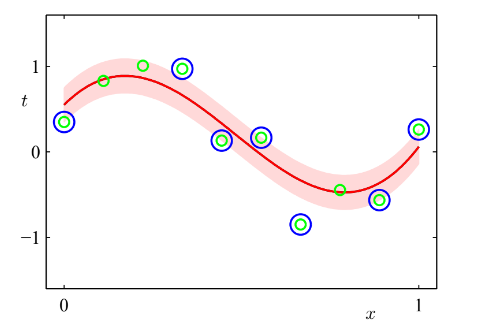
\includegraphics[width=15cm]{images/Kernel Methods/epsilon_tube.png}
    \label{fig:epsilon_tube}
\end{figure}

\chapter{Instance Based Learners}
\section{Instance Based Learners}
\subsection{Parametric vs Non-Parametric Models}

\textbf{Parametric models} have a fixed number of parameters. Examples:
\begin{itemize}
    \item Linear regression
    \item Logistic regression
    \item Perceptron
    \item \dots
\end{itemize}

\textbf{Non-parametric models}: Number of parameters grows with amount of data. 

A Simple non-parametric model is the instance-based learning.

\subsection{K-nearest neighbors}
It tries to solve the classification problem.

The classification with K-NN is as follows:
\begin{enumerate}
    \item Find K nearest neighbors of new instance x
    \item Assign to x the most common label among the majority of neighbors
\end{enumerate}

The likelihood of the class c for a new instance is given by:
\begin{equation}
    p(c|x, D, K) = \frac{1}{K} \sum_{x_{n} \in N_{k}(x_{n}, D)} I(t_{n} = c)
\end{equation}
with $N_{K}(x_{n}, D)$ the $K$ nearest points to $x_{n}$ and $I(e) = \{\begin{array}{lr}
        1 & \text{if e is true}\\
        0, & \text{if e is false}
        \end{array}$

We can change K to fit better the dataset and avoid overfitting.

\subsection{Kernelized nearest neighbours}
we can use a distance function in computing $N_{K}(x, D)$
\begin{equation}
    ||x-x_{n}||^{2} = x^{T}x + x^{T}_{n} - 2x^{T}x_{n}
\end{equation}
can be kernelized by using a kernel $k(x, x_{n})$

\subsection{Locally weighted regression}
Regression problem $f: X \xrightarrow{}\mathcal{R}$ with data set  $D = \{(x_{n}, t_{n})^{N}_{n=1}\}$. We can fit a local regression around a certain datapoint $x_{q}$.\\
We can firstly compute the K nearest neighbours of $x_{q}$, fit a regression on those neighbours and finally return $y(x_{q}; w)$. We can also use a kernelized regression.



\chapter{Multiple Learners}
\section{Multiple Learners}
Also called Ensemble Learning, is based on training many different learner/model and combine their result.

The general idea is that, if we use a baseline (single model) performances may be good, if we instead use bagging or voting (parallel) performances increases and if we use boosting (sequential) performance are even better.

\subsection{Voting}
Given a dataset $D$
\begin{enumerate}
    \item use $D$ to train a set of models $y_{m}(x)$, for $m = 1, \dots , M$
    \item make prediction with 
    \begin{equation}
        \begin{array}{lr}
             y_{voting}(x) = \sum w_{m}y_{m}(x) & \text{(regression)} \\
             y_{voting}(x) = \underset{c}{argmax}\sum w_{m}l(y_{m}(x)=c) & \text{weighted majority (classification)}
        \end{array}
    \end{equation}
\end{enumerate}
with the sum of $w_{m} = 1$, $l(e)=1$ if $e$ is true, 0 otherwise.\\
If we add a Non linear gating function $f$ depending on input, it is called \textbf{Mixture of experts}.\\
If we also try to learn the combination function $f$ it is called \textbf{Stakcing}.\\
\textbf{Cascading} learners are instead based on confidence threshold.\\
\\
\\
check coding scheme.\\
\\
\\
\subsection{Bagging}
Given a dataset $D$:
\begin{enumerate}
    \item generate M bootstrap data sets $D_{1} \dots D_{m}$, with $D_{i} \in D$.
    \item use each bootstrap data set $D_{m}$ to train a model $y_{m}(x)$, for each m.
    \item make predictions with a voting scheme
    \begin{equation}
        y_{bagging}(x) = \frac{1}{M} \sum y_{m}(x)
    \end{equation}
\end{enumerate}
\subsection{Boosting}
\subsubsection{general approach}
main points are:
\begin{itemize}
    \item Base classifiers (\textbf{weak learners}) trained \textbf{sequentially}
    \item Each classifier trained on weighted data
    \item Weights depend on performance of previous classifiers
    \item Points misclassified by previous classifiers are given greater weight. So that next models will classify better those points
    \item Predictions based on weighted majority of votes
\end{itemize}
\begin{figure}[H]
    \centering
    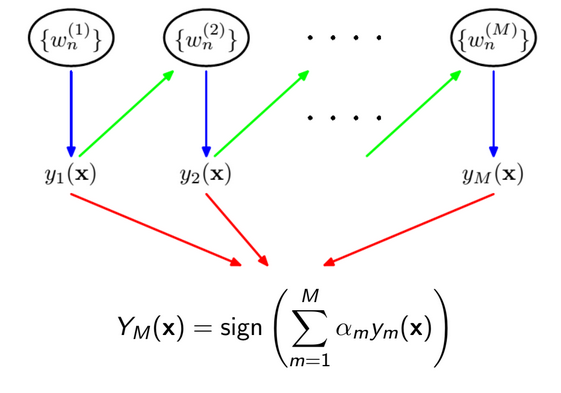
\includegraphics[width=15cm]{images/boosting/boosting.png}
    \label{fig:booting}
\end{figure}

\subsection{AdaBoost}
Given $D = \{(x_{1}, t_{1}), \dots, (x_{n}, t_{n})\}$, where $x_{n} \in X, t_{n} \in \{-1, +1\}$
\begin{enumerate}
    \item Initialize $w_{n}^{(m)}= 1/N,\ n=\, \dots, N$
    \item For $m=1, \dots, M$:
    \begin{itemize}
        \item Train a weak learner $y_{n}(x)$ my minimizing the weighted error function:
        \begin{equation}
            J_{m} = \sum_{n=1}*{N}w_{n}^{(m)}l(y_{m}(x_{n}) \neq t_{n})
        \end{equation}
        \item Evaluate: $\epsilon_{m} = \frac{\sum w_{n}^{(m)}l(y_{m}(x_{n}) \neq t_{n})}{\sum w_{n}^{(m)}}$ and $\alpha_{m}=\ln [\frac{1 - \epsilon_{m}}{\epsilon_{m}}]$
        \item Update the data weighting coefficients:
        \begin{equation}
            w_{n}^{(m+1)} = w_{n}^{(m)}exp[\alpha_{m}l(y_{m}(x_{n}\neq t_{n})]
        \end{equation}
    \end{itemize}
    \item Output the final classifier:
    \begin{equation}
        Y_{M}(x) = sign(\sum_{m=1}^{M}\alpha_{m}y_{m}(x))
    \end{equation}
\end{enumerate}
\begin{figure}[H]
    \centering
    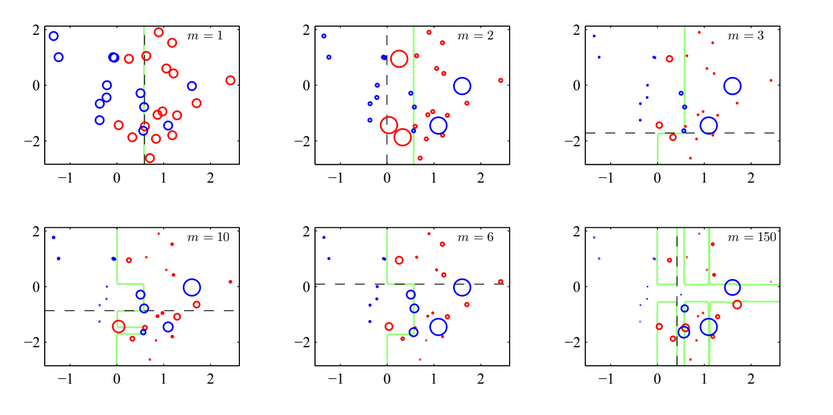
\includegraphics[width=15cm]{images/boosting/adaboost.png}
    \label{fig:adboost}
\end{figure}

\subsubsection{Exponential Error Minimization}
AdaBoosting can be explained as the sequential minimization of an exponential error function.\\
Consider the error function
\begin{equation}
    E = \sum_{n=1}^{N}exp[-t_{n}f_{M}(x_{n}],
\end{equation}
where $f_{M}$ is the final classifier
\begin{equation}
    f_{M}(x) = \frac{1}{2}\sum_{m=1}^{M}\alpha_{m}y_{m}(x),\ \ \ t_{n}\in \{-1, +1\}
\end{equation}
the goal is to minimize the error function $E$ w.r.t. $\alpha_{m}, y_{m}(x), m=1, \dots, M$

\textbf{Sequential minimization}, instead of minimizing $E$ \textit{globally}
\begin{itemize}
    \item assume $y_{1}(x), \dots, y_{M-1}(x)$ and $\alpha_{1}, \dots, \alpha_{M-1}$ fixed
    \item minimize w.r.t. $y_{M}(x)$ and $\alpha_{M}$.
\end{itemize}
Making $y_{M}(x)$ and $\alpha_{M}$ explicit we have:
\begin{equation}
    E=\sum_{n=1}^{N} exp[-t_{n}f_{M-1}(x_{n}) - \frac{1}{2}t_{n}\alpha_{M}y_{M}(x_{n}] = \sum w_{n}^{(M)}exp[-\frac{1}{2}t_{n}\alpha_{M}y_{M}(x_{n})]
\end{equation}
with $ w_{n}^{(M)} = exp[-t_{n}f_{M-1}(x_{n})]$ constant as we are optimizing w.r.t. $\alpha_{M}$ and $y_{M}(x)$

From sequential minimization we obtain $w_{n}^{(m+1)}$. Then we can predict with:
\begin{equation}
    sign(f_{M}(x)) = sign(\frac{1}{2}\sum \alpha_{m}y_{m}(x))
\end{equation}
which is equal to
\begin{equation}
    Y_{M}(x) =  sign(\sum \alpha_{m}y_{m}(x))
\end{equation}
thus providing that AdaBoost minimizes such error function

\subsubsection{AdaBoost: remarks}
Pros:
\begin{itemize}
    \item Fast and simple to implement
    \item no prior knowledge about base learners is required
    \item no parameters to tune
    \item can be combined with any method for finding best learners
    \item theoretical guarantees given sufficient data and base learners with moderate accuracy
\end{itemize}
Cons:
\begin{itemize}
    \item Performance depends on data and the base learners
    \item Sensitive to noise
\end{itemize}



\chapter{Artificial Neural Networks}
\section{Artificial Neural Networks}
With this chapter, the second part of the course begins.

\subsection{Problem}
We have $f: X \xrightarrow[]{}Y$, a dataset $D=\{(x, t)\}$, a model $\hat{f} (x; \Theta)$, an error function $E(\Theta)$, we want to minimize $\Theta^{*} = argmin E(\Theta)$ and predict the value of $x' \not\in D,\ \hat{f}(x', \Theta)$. The minimization will be tone through Iterative Linear Descent.

What is different from the previous models? $\hat{f}$ is non-linear both in the parameters and the dataset. So, NN provide non linear models in the set of parameters.

The second important aspect is that NN has the advantage that you don't have to specify a kernel. This is because kernels are automatically learned.

Alternative names are \textbf{Feedforward neural network} or \textbf{Multilayer perceptrons}. NN are function estimators and learn parameters so that the function \textbf{f} that they are learning approximates well the unknown function $f$.

\subsubsection{Inspiration}
NN were inspired by what we know of our brain. Note that they are not a model of the brain, but only comprehends some insights. Outputs can be seen as an array of units (neurons) activation based on the connections with the previous units. Feedforward NN are organized in layers, where each layer contains a set of neurons and each one is connected to every unit of the layer that follows. Information flows without any loop from the input to the output, passing through the hidden units.
\begin{equation}
    f(x; \Theta) = f^{3}(f^{2}(f^{1}(x; \Theta^{1}); \Theta^{2}); \Theta^{3})
\end{equation}
where $f^{i}$ is the i-th layer and $\Theta^{i}$ is the corresponding parameters.\\

The power of FNN is based on the fact that we don't have to handcraft kernels or to use a known one.\\
\subsection{XOR problem}
Consider the problem where we have a dataset: $D=\{((0, 0)^{T}, 0), ((0, 1)^{T}, 1), ((1, 0)^{T}, 1), ((1, 1)^{T}, 0),\}$ and we want to use the linear regression using the Mean Square Error (MSE). We can instantly notice that the datast is not linearly separable. If we use a linear model with a linear kernel it will not work. We could try a kernel, but with FNN we don't need to handcraft it.

We can build a two-layer network with two units as input layer, two units as hidden layer and one unit as output layer. We also have to define \textbf{activation function} These functions are present in any hidden layers as well as in the output layer. We can chose a different activation function for each layer. For this example we can use a \textbf{ReLU (rectified linear unit)} for the hidden layer and a linear activation function for the output layer.\\
\textbf{ReLU}: The ReLU units is a function that returns: $f(z)= max(0, z)$.\\
The i-th neuron of the hidden layer will have the form of:
\begin{equation}
    h_{i} = ReLU\left((w_{i,1}, w_{i,2})^{T} \begin{pmatrix} x_{i,1} \\ x_{i,2} \end{pmatrix} + w_{i,0}\right)
\end{equation}
we can then organize as a column vector each unit $h_{i}$ of the layer and rewrite as:
\begin{equation}
    h = \begin{pmatrix} h_{1} \\ h_{2}  \end{pmatrix} = ReLU\left(\begin{pmatrix} w_{1,1} & w_{1,2} \\ w_{2,1} & w_{2,2} \end{pmatrix} \begin{pmatrix}
        x_{1} \\ x_{2}
    \end{pmatrix} + \begin{pmatrix}  w_{1,0} \\ x_{2,0}
    \end{pmatrix}\right) = ReLU\left( W^{T}x + W_{0} \right)
\end{equation}

and so the ourpur of the model $y$ is
\begin{equation}
    y = w^{T} h + w_{0} = w^{t}ReLU\left( W^{T}x + W_{0} \right) + w_{0}
\end{equation}
We can now choose an error function. For instance, can use the MSE and minimize.

\subsection{Cost Function}
A model implicitly defines a conditional distribution $p(t| x, \Theta)$. This cost function is the Maximum likelihood principle (\textbf{cross-entropy}).
\begin{equation}
    J(\Theta) = E_{x, t\sim D} \left[-ln(p(t|x; \Theta))\right]
\end{equation}
For example we can assume the function to be a Gaussian distribution and hence use it to estimate and minimize the loglikelihood.

\subsection{Output units}
The choice of the loss function is related to the problem that we are modeling and to the output units of the network.
\begin{enumerate}
    \item Regression
    \item Binary Classification
    \item Multi-classes classification
\end{enumerate}

\textbf{Regression} \\
linear units: identity activation function.\\
\begin{equation}
    y = W^{T}h + b
\end{equation}
use a Gaussian distribution noise model
\begin{equation}
    p(t|x) = N(t|y, \beta ^{-1})
\end{equation}
\textit{Cost function} = maximum likelihood that is equal to the mean squared error.

\textbf{Binary classification} \\
Sigmoid units: sigmoid activation function.\\
The likelihood corresponds to a Bernoulli distribution.
\begin{equation}
\begin{multlined}
    J(\Theta) = E_{x, t \sim D}\left[-ln(p(t|x))\right] \\
    \textbf{where } -ln (p(t|x)) = softplus ((1 - 2t)\alpha) \\
    \textbf{with } \alpha = w^{T}h + b.
\end{multlined}
\end{equation}

\textbf{Multi-class Classification}
Uses Softmax units as activation function.
\begin{equation}
    y_{i} = softmax(\alpha_{i}) = \frac{exp(\alpha_{i})}{\sum exp (\alpha_{i})}
\end{equation}
And corresponds to a multinomial distribution:
\begin{equation}
    J_{i}(\Theta) = E_{x, t \sim D} \left[-\ln (softmax(\alpha_{i}))\right]
\end{equation}
with $\alpha_{i} = w^{T}_{i}h + x$

\subsubsection{Activation Functions for Hidden Units}
There is not a real rule. The choice is driven by intuition.
\begin{itemize}
    \item \textbf{ReLU}: rectified linear units
    \begin{equation}
        g(\alpha) = max(0, \alpha)
    \end{equation}
    easy to optimize but not differentiable on zero (does not cause problems in practice).
    \item \textbf{Sigmoid}: \begin{equation}
        g(\alpha) = \sigma(\alpha)
    \end{equation}
    \item \textbf{Hyperbolic tangent}:
    \begin{equation}
        g(\alpha) = tanh(\alpha)
    \end{equation}
    It is closely related to the sigmoid: $tanh(\alpha) = 2\sigma(2\alpha) - 1$
\end{itemize}
Do not use logaraithms since units saturate easily otherwise.Gradient based learning is very slow. $tanh$'s gradient is larger than sigmoid's one.


\subsection{Gradient computation}
Information flows forward through the network while computing network output $y$ from input $x$.

To train the parameters we need to compute gradients wrt the network parameters $\Theta$.

The \textbf{backpropagation} algorithm propagates the information back from the output to the whole network.

Backpropoagation is not specific to FNNs and is not a training algorithm. It only used for computing the gradients.

\subsubsection{Chain rule}
The chain rule is the core of backpropagation:
\begin{equation}
    \frac{dz}{dx} = \frac{dz}{dy}\frac{dy}{dx}
\end{equation}
and for vector functions the rule is:
\begin{equation}
    \frac{\partial z}{\partial x_{i}} = \sum_{j}\frac{\partial z}{\partial y_{j}}\frac{\partial y_{j}}{\partial x_{i}}
\end{equation}
The equivalent in vector notation is:
\begin{equation}
        \nabla_{x}z = \left(\frac{\partial y}{\partial x}\right)^{T} \nabla_{y}z
\end{equation}
with $\frac{\partial y}{\partial x}$ the $n \times m$ Jacobian matrix of g.

\subsubsection{Backpropagation algorithm}

\begin{figure}[H]
    \centering
    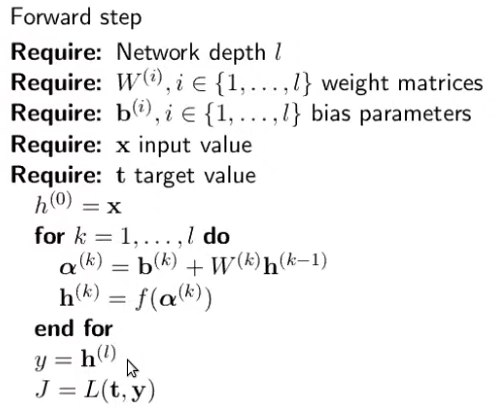
\includegraphics[width=15cm]{images/FNN/backprop_forward_Step.png}
    \caption{Forward step}
    \label{fig:forw_step}
\end{figure}

\begin{figure}[H]
    \centering
    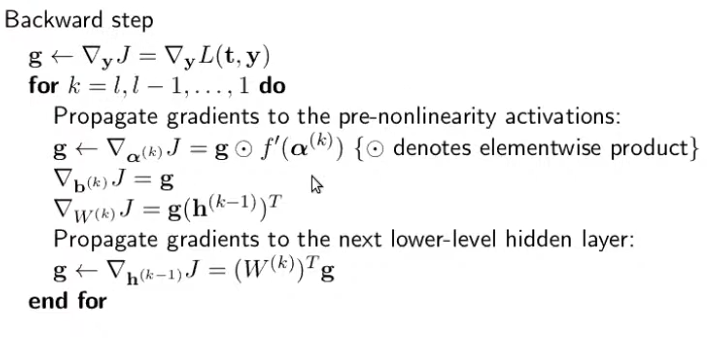
\includegraphics[width=15cm]{images/FNN/backprop_backward_Step.png}
    \caption{Backward step}
    \label{fig:backw_step}
\end{figure}

\textbf{Note}: this algorithm is specific for MLPs. This algorithm can also be optimized through caching.

\subsection{Learning Algorithms}
\subsubsection{SGD}

\begin{figure}[H]
    \centering
    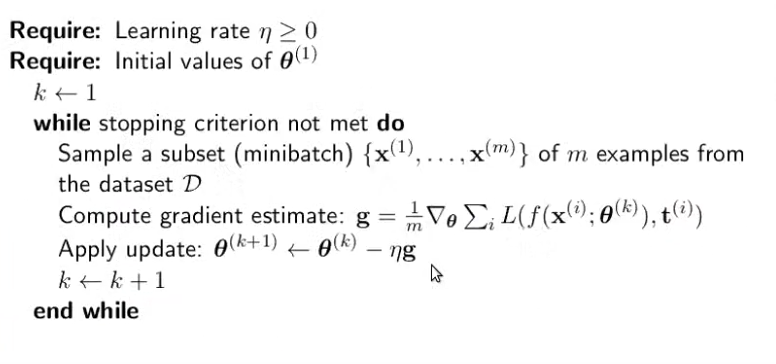
\includegraphics[width=15cm]{images/FNN/SGD.png}
    \caption{SGD algorithm. The gradient is calculated through the backpropagation.}
    \label{fig:sgd}
\end{figure}

We change $\eta$ according to some rules through iterations.

Until iteration $\tau$:
\begin{equation}
    \eta^{(k)} = \left(1 - \frac{k}{\tau}\right)\eta^{(k)} + \frac{k}{\tau}\eta^{(\tau)}
\end{equation}
after iteration $\tau$ we have $\eta^{(k)} = \eta^{(\tau)}$

\subsubsection{SGD with momentum}
\begin{figure}[H]
    \centering
    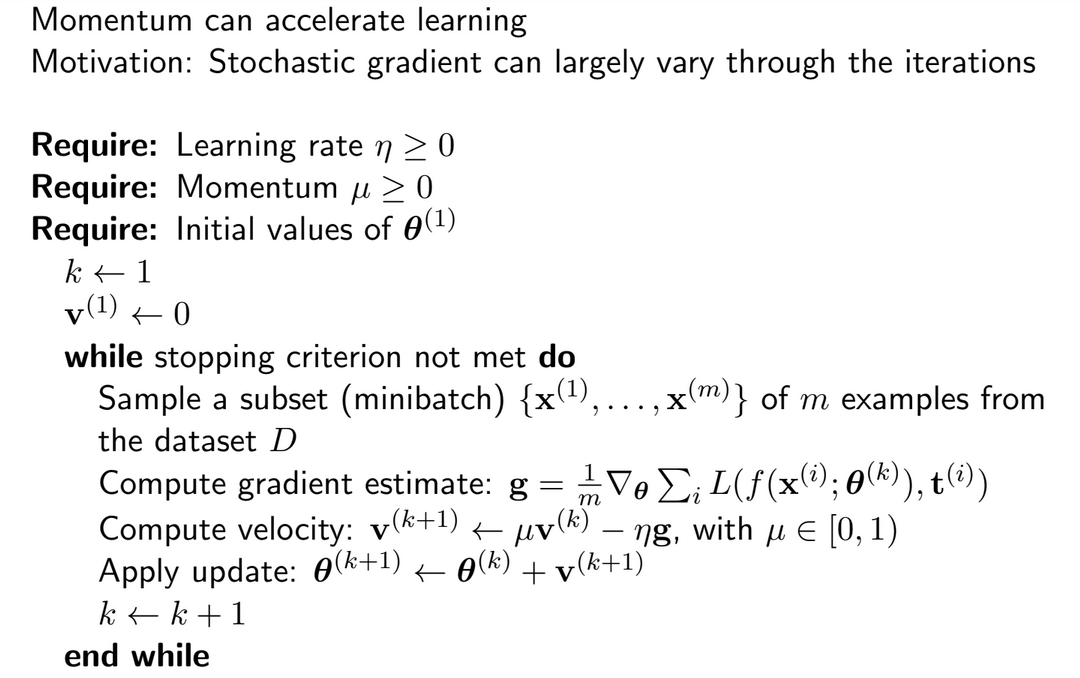
\includegraphics[width=15cm]{images/FNN/SGD_momentum.png}
    \caption{SGD algorithm with momentum. The gradient is calculated through the backpropagation.}
    \label{fig:sgd_momentum}
\end{figure}
Momentum helps overcome local minimums. It starts an oscillation movement when he reaches a minimum.

SGD with \textbf{Nestov} momentum is another technique that consists in applying the momentum before computing the gradient. This technique sometimes improves the convergence rate.

\subsubsection{Adaptive learnings}
Based on th eanalisys of the gradient of the loss function it's possible to determine, at any step algorithm, whether the learning rate should be increased or decreased.

Some examples of adaptive learning rates are:
\begin{itemize}
    \item AdaGrad
    \item RMSProp
    \item Adam
\end{itemize}


\subsection{Architectural Design}
What can we chose of a FNN?
\begin{itemize}
    \item Depth
    \item Width of a layer
    \item Activation functions
    \item Loss function
\end{itemize}

The \textbf{Universal Approximation Theorem} does not say how to set these parameters.

For the output of the neural network we can use the softmax if we have to classify the datapoint. The softmax will be translated into a one-hot encoding ({1, 0, 0}, {0, 1, 0}, ...) or in a Categorical encoding ({1, 2, 3}).\\
for the loss function we have two formats of the output: Categorical Cross Entropy vs Sparse categorical cross entropy.

How do we calculate the number of parameters for a Fully connected layer?
if we have $a$ layers as input and the next layer has $b$ units we can calculate the number of parameters as: $a \times b + b = (a + 1) \times b$. We can calculate the number of parameters for each Fully connected layer and sum the values to get the total number of parameters.



\subsection{Regularization}
Regularizatoin is an important step for FNN too if we want to reduce overfitting.\\
We have different options for FNN:
\begin{itemize}
    \item Parameter norm penalties
    \item Dataset argumentation
    \item Early stopping
    \item Parameter sharing
    \item Dropout
\end{itemize}

If the network improves the accuracy on Training set but not on Test set then the network is overfitting.

\subsubsection{Parameter norm penalties}
We can penalize high absolute values of the parameters:
\begin{equation}
    E_{reg}(\Theta) = \sum_{j} |\Theta_{j}|^{q}
\end{equation}
resulting in the cost function:
\begin{equation}
    \overline{J}(\Theta) = J(\Theta) + \lambda E_{reg}(\Theta)
\end{equation}

Programming Libraries usually let you choose a $\lambda$ for each layer. If the value is not set, il will be set to $0$ and the parameters will not be penalized.

\subsubsection{Dataset Argumentation}
We can generate new datapoint and include them in the dataset.
\begin{itemize}
    \item Data Transformation
    \item Adding noise
\end{itemize}

\subsubsection{Early Stopping}
We can stop iterations early to avoid overfitting. In order to know when to stop we can use cross-validation to determine the best values. We can also send different training run with random initialization values, where each run will evolve differently an maybe one of them will have a better accuracy.

\subsubsection{Parameter sharing}
Parameter sharing consists in setting constraints on having subset of model parameters to be equal.

In CNNs this method allows for invariance to translation.

\subsubsection{Dropout}
Randomly ignore network units with some probability $\alpha$. So I will apply the algorithm only on a subset of connection (for a single step). I can apply dropout to every step an randomly ignore a different random subset of parameters at each iteration.

\subsection{Convolutional Neural Networks}

\subsection{Motivation}
Up to now we treated inputs as general feature vectors. In some cases they have a special structure:
\begin{itemize}
    \item Audio
    \item Images
    \item Videos
\end{itemize}

Signals are a numerical representation of physical quantities. Deep learning can be directly applied on signals by using suitable operations.

We cannot simply flatten the input because images, audio and videos have a semantics that cannot be ignored. By flatting the input we loose information and consequently the network will not behave well.

\subsubsection{Convolution}
Given an image $I$ and a kernel $K$, the 2-D convolution is:
\begin{equation}
    (I*K)(i,j) \equiv \sum_{m \in S_{1}}\sum_{n \in S_{2}} I(m, n)K(i-m, j-n)
\end{equation}
where $S_{i}$ are finite sets.
for a 3-D convolution the formula is:
\begin{equation}
        (I*K)(i,j, k) \equiv \sum_{m \in S_{1}}\sum_{n \in S_{2}}\sum_{u \in S_{3}} I(m, n, u)K(i-m, j-n, k-u)
\end{equation}
Properties: 
\begin{itemize}
    \item convolution is commutative: $(I*K)(i, j) = (K*I)(i, j)$
    \item Cross-correlation: we can flip the kernel and modify the convoution
    \begin{equation}
        (I*K)(i,j) \equiv \sum_{m \in S_{1}}\sum_{n \in S_{2}} I(i+m, j+n)K(m, n)
    \end{equation}
\end{itemize}

\subsubsection{Different types of Convolution}
based on the direction of the movement of the kernel, the convolution can be 1D, 2D, 3D...\\
So it is based on the degree of freedom of the kernel.

Convolution changes the shape of the tensor.

\subsubsection{Padding}
We can add a padding in order to convolve and keep the size of the image. Padding can be all zeros

\subsection{Terminology}
\begin{itemize}
    \item Input size
    \item Kernel size
    \item Feature map or Depth slice: output of convolution between an input and one kernel
    \item Depth: number of kernels
    \item Padding
    \item Stride: step of sliding kernel
    \item Receptive field: region in the input space that a particular feature is looking at.
\end{itemize}

\subsubsection{Convolutional Layers}
Are usually made up by three layers:
\begin{itemize}
    \item Convolution between input and kernel
    \item non-linear activation function
    \item pooling
\end{itemize}

For the detector stage we use one of the same that we use for FNNs.

\subsubsection{Properties of CNNs}
Sparse interaction/connectivity: brings in the concept of locality.
Parameter sharing: constraint on values of the kernels.

Pooling stage implements invariance to local translations. Some frequently used pooling layers are \textbf{maxpooling} and \textbf{average pooling}. When applied with stride it reduces the size of the output layer (\textbf{subsampling}).

\subsubsection{Calculate the feature map size}
Consider the input size $w_{in} \times h_{in} \times d_{in}, d_{out}$ kernels of size $w_{k} \times h_{k} \times d_{in}$, stride $s$ and padding $p$, the dimension of the feature map can be calculated as:
\begin{equation}
    w_{out} = \frac{w_{in} - w_{k} + 2p}{s} + 1
\end{equation}
\begin{equation}
    h_{out} = \frac{h_{in} - k_{k} + 2p}{s} + 1
\end{equation}

while the number of trainable parameters is: 
\begin{equation}
    |\Theta| = w_{k} \cdot h_{k} \cdot d_{in} \cdot d_{out} + d_{out}
\end{equation}

\subsection{Networks for Images}

\textbf{}{LeNet} is a simple but yet good neural network composed of 7 layers.
The input is a $32 \times 32$ image and the output are 10 neurons (10 classes).

Other famous neural networks (not deep) are:
\begin{itemize}
    \item ResNet
    \item VGG
    \item GoogLeNet
    \item AlexNet
\end{itemize}

\subsection{Transfer Learning}
The idea is to understand how to exploit learning on a different task for learning on a new task.\\
$D$ is a domain defined by data points $x_{i} \in X$, distributed according to $D(X)$. $T$ is a learning task defined by labels $y \in Y$, a target function $f: X \xrightarrow[]{} Y$, and distribution $P_{D}(y|x)$.\\
Given:
\begin{itemize}
    \item $D_{T}$ and $T_{S}$ a source domain learning task
    \item $D_{T}$ and $T_{T}$ a target domain learning task
    \item in general $D_{S} \neq D_{T}$ and $T_{S} \neq T_{T}$
\end{itemize}
Our goal is to improve learning of $f_{T}: X_{T} \xrightarrow[]{} Y_{T}$ using knowledge in $D_{S}$ and $DT_{S}$.

\subsubsection{Solutions}
\textbf{Fine-tuning}: Use the same architecture (or part of it) and initialize it with the pretrained models. Then you can:
\begin{itemize}
    \item train of all network parameters
    \item freeze parameters of some layers.
    \begin{itemize}
        \item \textbf{Pros}: Full advantage of CNNs.
        \item \textbf{Cons}: 'Heavy' training.
    \end{itemize}
\end{itemize}

\textbf{CNN as feature extractor}: We use a CNN as a feature extractor network, usually by cutting the last layers and by then using a flatten/dense layer. Then we train a new classifier based on those extracted features.
\begin{itemize}
        \item \textbf{Pros}: No need to train CNNs.
        \item \textbf{Cons}: Cannot modify features
\end{itemize}


\chapter{Unsupervised Learning}
\section{Unsupervised Learning}
We want to learn a distribution without knowing the labels. This is considered a more complex and difficult problem than supervised learning.
\begin{equation}
    \begin{multlined}
        f: X \xrightarrow{} Y \\
        D = \left\{ (x_{n}) \right\}
    \end{multlined}
\end{equation}
\subsection{Gaussian Mixture Model}
We assume that the dataset is generated by a probability distribution which is the sum of different Gaussian functions:
\begin{equation}
    P(x) = \sum_{k=1}^{k}\pi_{k}N\left(x; \mu_{k}, \Sigma_{k}\right)
\end{equation}
Where $\pi_{k}$ is the prior probability, $\mu_{k}$ is the mean and $\Sigma_{k}$ is the covariance matrix.\\
When we have these information we can easily generate datapoints by sampling the distribution. We firstly select one of the Gaussians based on the probability $\pi$ and then we sample it.

\subsection{K-means}
Now that we know how to sample from a GMM, we can try to find the means of the distributions.

The K-means algorithm tries to find the K centroids of the K Gaussians.\\
The iterative process of the algorithm is the following:
\begin{enumerate}
    \item Begin with a decision on the number of clusters (k)
    \item Initialize the positions of the means. You may assign the training samples randomly, or systematically as follows
    \begin{itemize}
        \item Take the first k training samples as single element cluster
        \item Assign each of the remaining (N - k) training samples to the cluster with the nearest centroid. After each assignment, recompute the centroid of the new cluster.
    \end{itemize}
\end{enumerate}
The algorithm stops when there are no changes in the assignment.\\
The algorithm converges because:
\begin{itemize}
    \item At each switch in step 2, the distance between the points and the centroids is decreased.
    \item There are only a finite number of partitions that assign data points to k clusters.
\end{itemize}

\textbf{Cons} of K-means:
\begin{itemize}
    \item The number of K must be decided before hand. There are algorithms that tries to find the best K.
    \item Sensitive to initial condition (local optimum) when a few data available. 
    \item Not robust to outliers
    \item the result is a circular cluster shape because it is based on distance.
\end{itemize}
Some improvements to K-means:
\begin{itemize}
    \item Use it only if there are many data available
    \item use median instead of mean
    \item define better distance functions.
\end{itemize}

\subsection{Predict GMM}
A different way of predicting the GMM is by introducing a latent variable $z_{k} \in \left\{0, 1\right\}$., with $z = \left(z_{1}, \dots, z_{k}\right)$ and 1-out-of-K encoding.\\
Let's define
\begin{equation}
    P(z_{k} = 1) = \pi_{k}
\end{equation}
\begin{equation}
    P(z_{k}) = \sum_{k=1}^{K}\pi_{k}^{z_{k}}
\end{equation}
For a given value of $z$:
\begin{equation}
    P(x|z_{k} = 1) = N(x; \mu_{k}, \Sigma_{k})
\end{equation}
thus
\begin{equation}
    P(x|z) = \prod_{k=1}^{K}N(x; \mu_{k}, \Sigma_{k})^{Z_{k}}
\end{equation}
Joint distribution: $P(x, z) = P(x|z)P(z)$ (chain rule).\\
When $z$ are variables with 1-out-of-K encoding and $P(z_{k} = 1) = \pi_{k}$,
\begin{equation}
\label{abc}
    P(x) = \sum_{z}P(z)P(x|z) = \sum_{k=1}^{K}\pi_{k}N(x; \mu_{k}, \Sigma_{k})
\end{equation}
GMM distribution can be seen as the maximization of $P(x, z)$ over variables $z$. By reversing the equation \ref{abc} we can learn the GMM.

Let's define the \textbf{posterior} 
\begin{equation}
    \begin{multlined}
        \gamma(z_{k}) \equiv P(z_{k} = 1 | x) = \frac{P(z_{k} = 1)P(x|z_{k} = 1)}{P(x)} = \\
        \frac{\pi_{k}N(x;\mu_{k}, \Sigma_{k})}{\sum_{j=1}^{K}\pi_{j}N(x;\mu_{j}, \Sigma_{j})}
    \end{multlined}
\end{equation}

\subsection{Expectation Maximization (EM)}
It is a general iterative algorithm based on two steps: \textbf{Expectation} and \textbf{Maximization}.\\
The algorithm computes the maximum likelihood 
\begin{equation}
    \underset{params}{argmax}P(X|params)
\end{equation}

Expectation maximization consists of:
\begin{itemize}
    \item \textbf{E step}: Given $\pi_{k}, \mu_{k}\text{, and } \Sigma_{k}$ compute $\gamma(Z_{nk})$
    \item \textbf{M step}: Given $\gamma(Z_{nk})$, compute $\pi_{k}, \mu_{k}\text{, and } \Sigma_{k}$
\end{itemize}

\subsubsection{EM for GMM}
\begin{equation}
    \begin{multlined}
        \mu_{k} = \frac{1}{N_{k}}\sum_{n=1}^{N}\gamma(z_{nk})x_{n}\\
        \Sigma_{k} = \frac{1}{N_{n}}\sum_{n=1}^{K}\gamma(z_{nk})(x_{n}-\mu_{k})(x_{n}-\mu_{k})^{T}\\
        \pi_{k} = \frac{N_{k}}{N}\text{, with }N_{k}=\sum_{n=1}^{N}\gamma(z_{nk})
    \end{multlined}
\end{equation}

The algorithm for GMM:
\begin{itemize}
    \item Initialize $\pi_{k}^{(0)}, \mu_{k}^{(0)}\text{, and } \Sigma_{k}^{(0)}$
    \item repeat until termination condition:
    \begin{itemize}
        \item \textbf{E step}
        \begin{equation}
            \gamma(z_{nk})^{(t + 1)} = \frac{\pi_{k}^{(t)}N(x;\mu_{k}^{(t)}, \Sigma_{k}^{(t)})}{\sum_{j=1}^{K}\pi_{j}^{(t)}N(x;\mu_{j}^{(t)}, \Sigma_{j}^{(t)})}
        \end{equation}
        \item \textbf{M step}
        \begin{equation}
            \begin{multlined}
                \mu_{k}^{(t + 1)} = \frac{1}{N_{k}}\sum_{n=1}^{N}\gamma(z_{nk})^{(t + 1)}x_{n}\\
                \Sigma_{k}^{(t + 1)} = \frac{1}{N_{n}}\sum_{n=1}^{K}\gamma(z_{nk})^{(t + 1)}(x_{n}-\mu_{k}^{(t + 1)})(x_{n}-\mu_{k}^{(t + 1)})^{T}\\
                \pi_{k}^{(t + 1)} = \frac{N_{k}}{N}\text{, with }N_{k}=\sum_{n=1}^{N}\gamma(z_{nk})^{(t + 1)}
            \end{multlined}
        \end{equation}
    \end{itemize}
\end{itemize}
Notice that if we consider only $\mu$, this is the same as K-means.

\subsubsection{General EM problem}
Given observed data, an unobserved latent variable and a parameterized probability distribution $P(Y|\Theta)$, where $\Theta$ are the parameters

Em in general converges to a local optimum. It provides an estimation for the latent variables.

EM has many uses in Unsupervised clustering, Bayesian Networks and Hidden Markov Models.

The method is the following: Given a likelihood function $Q(\Theta'|\Theta)$ which calculates $Y = X \cup Z$, the algorithm is:
\begin{enumerate}
    \item \textbf{Estimation step}: Calculate $Q(\Theta'|\Theta)$ using current hypothesis $\Theta$ and observed data $X$ to estimate probability distribution over $Y$
    \begin{equation}
        Q(\Theta'|\Theta) \xleftarrow{} E[\ln P(Y|\Theta')|\Theta, X]
    \end{equation}
    \item \textbf{Maximization step}: Replace hypothesis $\Theta$ by the hypothesis $\Theta'$ that maximizes the $Q$ function
    \begin{equation}
        \Theta \xleftarrow{} \underset{\Theta'}{argmax} Q(\Theta'|\Theta)
    \end{equation}
\end{enumerate}




\chapter{Bayesian Network}
\section{Bayesian Network}
The syntax of a Bayesian network is the following:
\begin{itemize}
    \item a set of nodes, one per variable
    \item a direct, \textbf{acyclic} graph
    \item a conditional distribution for each node given its parents.
\end{itemize}

It is a Probability Graphical Model (PBG). We use a Condition Probability Table (CPT) to represent causes and effects. Given the parents of the node $X_{i}$, he is independent from all the other variables. I only have to express $P(X_{i} | Parents(X_{i})$.

Consider a set of rules: $A\xrightarrow{}C$, $B\xrightarrow{}C$, $B\xrightarrow{}E$, $C\xrightarrow{}E$, $C\xrightarrow{}D$. Instead of having $P(A, B, C, D, E)$, I can use: $P(A)$, $P(B)$, $P(C|A,B)$, $P(E|B,C)$ and $P(D|C)$. We can use the chain rule to calculate probabilities:
\begin{figure}[H]
    \centering
    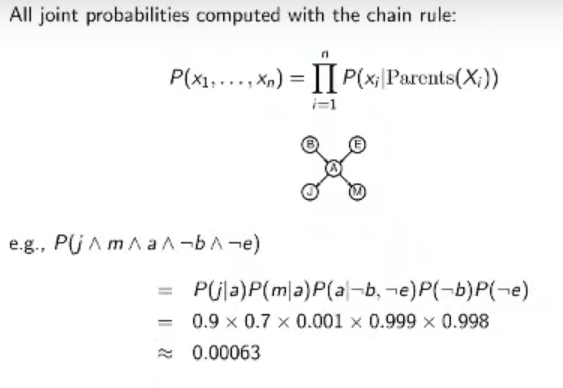
\includegraphics[width=7cm]{images/BayesianNetwork/Bayesian_Networks.png}
    \caption{Caption}
    \label{fig:Bayesian_networks}
\end{figure}

We can use the parameters $\Theta = <\Theta_{1}, \dots, \Theta_{n}>$ and calculate the inference. In machine learning we are interested in learning these parameters given a dataset.

If we can observe every variable it is easy since we can count the number of times that each variable is true/false and infer probabilities:
\begin{equation}
    P(A=1 | B = 0) \approx \frac{|\{d_{k} = \langle a_{k}, x_{k}, \dots\rangle \}| a_{k} = 1 \And x_{k} = 0|}{|\{d_{k} | x_{k} = 0|\}}
\end{equation}

If we have an unknown variable $X$ we can define $\Theta_{1} \dots \Theta_{n}$ as $P(X = 0) = \Theta_{0}$, $P(A = a_{1} | X = 0) = \Theta_{1}$, $P(A = a_{1} | X = 1) = \Theta_{2}$, $P(B = b_{1} | X = 0) = \Theta_{3}$, $P(B = b_{1} | X = 1) = \Theta_{4}$, $\Theta = \langle \Theta_{0}, \Theta_{1}, \Theta_{2}, \Theta_{3}, \Theta_{4} \rangle$ and use EM algorithm to maximize $\Theta$ from $D = \{(a_{1}, b_{1}), \dots, (a_{k}, b_{k})\}$.

Estimation:
\begin{equation}
    \begin{multlined}
        P(X = x_{j}) = \frac{1}{N} E [\hat{N}(X = x_{j})] \\
        P(A = a_{j} | X = x_{j}) = \frac{E[\hat{N}(A = a_{j}, X = x_{j})]}{E[\hat{N}(X = x_{j}]}
    \end{multlined}
\end{equation}
Maximization:
\begin{equation}
    E[\hat{N}(\cdot)] = E\left[\sum_{k}I(\cdot|d_{k})\right] = \sum_{k} P(\cdot | d_{k})
\end{equation}

\chapter{Dimensionality}
\section{Dimensionality Reduction}
\subsection{Latent Variables}
Sometimes not every information that we have from the input is important. Data may lie in a different lower dimension.
\begin{figure}[H]
    \centering
    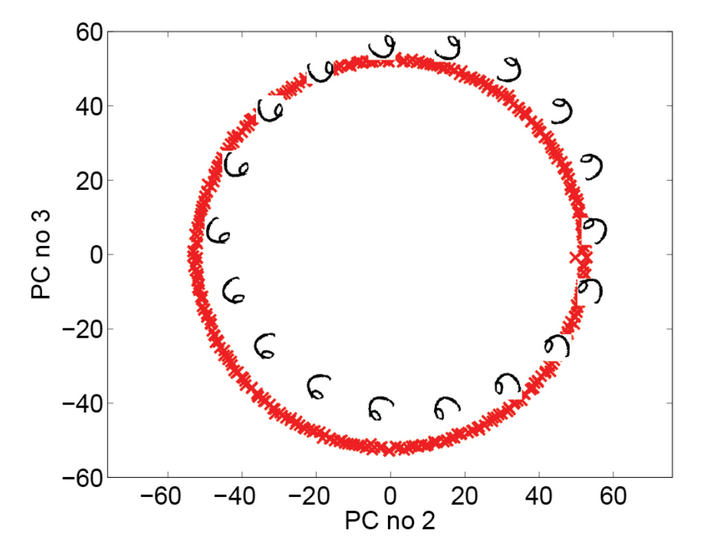
\includegraphics[width = 15cm]{images/DimRed/Manifold.png}
    \caption{Manifold that represents the rotation of a digit}
    \label{fig:manifold}
\end{figure}
This is usually possible for images since they have a structure and a semantic segmentation.

For data with structure we expect fewer distortions than dimensions and data usually live on a lower dimensional manifold. As a conclusion, we can deal with high dimensional data by looking for lower dimensional embeddings.

\subsubsection{PCA}
PCA is a method for dimension reduction that aims to maximize data variance after projection to some direction $u_{1}$. Projection points are:
\begin{equation} \label{projection}
    u_{1}^{T}x_{n}
\end{equation}
note that $u_{1}^{T}u_{1} = 1$

\begin{figure}[H]
    \centering
    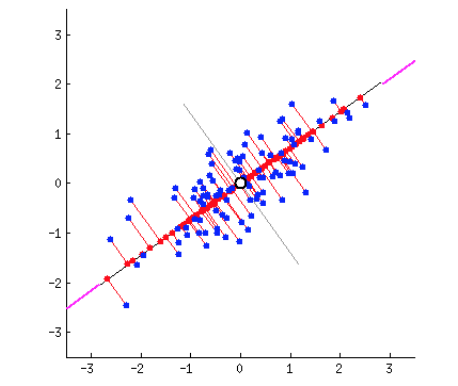
\includegraphics[width=10cm]{images/DimRed/pca.png}
    \caption{PCA variance maximization}
    \label{fig:pca}
\end{figure}

The first thing that we do is find the mean value of datapoints
\begin{equation}
    \overline{x} = \frac{1}{N}\sum_{n=1}^{N}x_n 
\end{equation}
and the data-centered matrix is:
\begin{equation}
    X=\begin{bmatrix}
    (x_{1} - \overline{x})^{T} \\ \dots \\ (x_{n} - \overline{x})^{T} \\ \dots \\ (x_{N} - \overline{x})^{T}
    \end{bmatrix}
\end{equation}
PCA is able to reduce \textbf{ONLY} to linear transformations. There are some techniques that are able to find non linear projections.
Now that data is normalized, we can find the linear projection that maximize the data. The projection point can be calculated as shown in \ref{projection}. If we apply the projection on every point, we have
\begin{equation}
    D = \langle u_{1}^{T}x_{n}, \dots, u_{1}^{T}x_{n}, \dots, u_{D}^{T}x_{n}\rangle
\end{equation}
now that we know how to apply the projection of points on a direction, we have to find which are the best directions. the mean of the projected points is $u_{1}^{T}\overline{x}$ and the variance of the projection points is:
\begin{equation}
\label{variance_of_projection}
    \frac{1}{N} \sum_{n=1}^{N}[u_{1}^{T}x_{n} - u_{1}^{T}\overline{x}]^{2} = u_{1}^{T}Su_{1}
\end{equation}
with
\begin{equation}
\label{cov_mat_norm}
    S = \frac{1}{N}\sum_{n=1}^{N}(x_{n} - \overline{x})(x_{n} - \overline{x})^{T} = \frac{1}{N}X^{T}X
\end{equation}
note: $S$ (\ref{cov_mat_norm}) is equal to the covariance normalized matrix, while \ref{variance_of_projection} is just a matrix multiplication on left and right of $S$ by $u_{1}$ (the left one is transposed).

If we try to maximize this value we get:
\begin{equation}
    \underset{u_{1}}{max}\ u_{1}^{T}Su_{1}
\end{equation}
subject to $u_{1}^{T}u_{1} = 1$. This is equivalent to unconstrained maximization with a Lagrange multiplier
\begin{equation}
    \underset{u_{1}}{max}\ u_{1}^{T}Su_{1} + \lambda_{1}(1 - u_{1}^{T}u_{1})
\end{equation}
and the solution is reached by setting the derivative w.r.t. $u_{1}$ to zero:
\begin{equation}
    Su_{1} = \lambda_{1}u_{1}
\end{equation}
where $u_{1}$ must be an eigenvector if $S$.

Left-multiplying by $u_{1}^{T}$ and using $u_{1}^{T}u_{1} = 1$, we have
\begin{equation}
    u_{1}^{T}Sy_{1} = \lambda_{1}
\end{equation}
which is the variance after the projection. In general, S will have different eigenvalues and eigenvectors. The eigenvalues that maximize the projections are the ones with an higher value. so, the first vector that will maximize the projection is the one associated to the highest eigenvalue, the second one will be the one associated to the second highest value, and so on.

\textbf{PCA Error minimization}: Consider a complete orthonormal D-dimensional basis such that
\begin{equation}
    u_{i}^{T}u_{j} = \delta_{ij}
\end{equation}
with
\begin{equation}
    \delta_{ij} =
    \begin{cases}
      1 \text{ if } i = j\\
      0 \text{ otherwise}
    \end{cases}
\end{equation}
Each datapoint can be written as 

\begin{equation}
    x_{n} = \sum_{i=1}^{d}\alpha_{ni}u_{i}
\end{equation}
using the orthonormal property we have $\alpha_{ni} = x_{n}^{T}u_{i}$, hence
\begin{equation}
    x_{n} = \sum_{i=1}^{d}(x_{n}^{T}u_{i})u_{i}
\end{equation}
the goal is to approximate $x_{n}$ using a lower-dimensional representation. We can write
\begin{equation}
    \Tilde{x}_{n} = \sum_{i=1}^{m}z_{ni}u_{i} + \sum_{i=m+1}^{d}b_{i}u_{i}
\end{equation}
Note: $b_{i}$ terms do not depend on sample $x_{n}$. \\
Evaluate approximation error (MSE) as
\begin{equation}
    J = \frac{1}{N}\sum_{n=1}^{N}||x_{n} - \Tilde{x}_{n}||^{2}
\end{equation}
Minimizing wrt $z_{nj}$ and $b_{i}$, we get:
\begin{equation}
    \begin{multlined}
        z_{ni} = x_{n}^{T}u_{i}\text{, } i= 1, \dots, m \\
        b_{i} = \overline{x}^{T}u_{i}\text{, } i= M + 1, \dots, d
    \end{multlined}
\end{equation}

Using these expression we get
\begin{equation}
    x_{n} - \Tilde{x}_{n} = \sum_{i=m+1}^{d} [(x_{n} - \overline{x})^{T}u_{i}]u_{i}
\end{equation}
The overall approximation error becomes
\begin{equation}
    J = \frac{1}{N}\sum_{n=1}^{N}\sum_{i=m+1}^{d}(x_{n}^{T}u_{i} - \overline{x}^{T}u_{i})^{2} = \sum_{i=m+1}^{d}u_{i}^{T}Su_{i}
\end{equation}

Minimize the approximation error subject to constraint $u_{i}^{T}u_{i} = 1$:
\begin{equation}
    \Tilde{J} = \sum_{i=m+1}^{d}u_{i}^{T}Su_{i} + \lambda_{i}(1 - u_{i}^{T}u_{i})
\end{equation}
If we set the derivative of a $u_{i}$ to zero, we get the exact same mathematical problem that we have found before:
\begin{equation}
    Su_{i} = \lambda_{i}u_{i}
\end{equation}
hence $u_{i}$ is an eigenvector of $S$ with eigenvalue $\lambda_{i}$. The approximation error is then given by:
\begin{equation}
    J = \sum_{i=m+1}^{d}\lambda_{i}
\end{equation}
and this is minimized by selecting $u_{i}$ as the eigenvectors corresponding to the $d - m$ smallest eigenvalues. In other words, the error is the sum of those last eigenvectors that we do not consider.

If we have less samples than dimensions, PCA is inefficient. a trick that we can use in this case is letting X be the $N\times d$ centered data matrix (i.e., n-th row is $(x_{n}-\overline{x})^{T}$) and the corresponding covarinace matrix:
\begin{equation}
    S = \frac{1}{N}X^{T}X
\end{equation}
the corresponding eigenvector equation is
\begin{equation}
    \frac{1}{N}X^{T}Xu_{i} = \lambda_{i}u_{i}
\end{equation}
By left multiplying by X we obtain:
\begin{equation}
    \frac{1}{N}XX^{T}(Xu_{i}) = \lambda_{i}(Xu_{i})
\end{equation}
and if we define $v_{i} = Xu_{i}$ we have
\begin{equation}
    \frac{1}{N}XX^{T}v_{i} = \lambda_{i}v_{i}
\end{equation}
so we have $XX^{T}$ which has the same $N - 1$ eigenvalues of $X^{T}X$ and is a $N\times N$ matrix whose eigenvalues can be computed efficiently.

given the eigenvalues $\lambda_{i}$ of $XX^{T}$, to find the eigenvectors we left-multiply by $X^{T}$
\begin{equation}
    \left(\frac{1}{N}XX^{T}\right)\left(X^{T}v_{i}\right) = \lambda_{i}\left(X^{T}v_{i}\right)
\end{equation}
This makes clear that $\left(X^{T}v_{i}\right)$ is an eigenvector of $S$ with eigenvalue $\lambda_{i}$. To find the direction $u_{i}$ we have to normalize the eigenvectors such that $u_{i}^{T}u_{i} = 1$:
\begin{equation}
    u_{i} = \frac{1}{\sqrt{N\lambda_{i}}} X^{T}v_{i}
\end{equation}

\textbf{Linear latent variable model}:
\begin{itemize}
    \item Represent data x with lower dimensional latent variables z
    \item Assume linear relationship $x = Wx + \mu$
    \item Assume Gaussian distribution of latent variables z $P(z) = N(z; 0, I)$
    \item Assume Linear-Gaussian relationship between latent variables and data $P(x|z) = N(x;Wz + \mu, \sigma^{2}I)$    
\end{itemize}
So, \textbf{Probabilistic PCA} is a model that, given the dataset, estimates the parameters of the models ($W, z$ and $\sigma$). we can setup a Maximum Likelihood that, given data $X$, sets the derivative of 
\begin{equation}
    \underset{W, \mu, \sigma^{2}}{argmax} \ln P(X|W, \mu, \sigma^{2}) = \sum_{n=1}^{N} \ln P(x_{n}|W, \mu, \sigma^{2})
\end{equation}
 to zero and finds the parameters of the model that, given z will generate a sample x.

\subsection{non-Linear Latent Variable Models}
Sometimes, linear representations are not sufficient for complex data
\begin{figure}
    \centering
    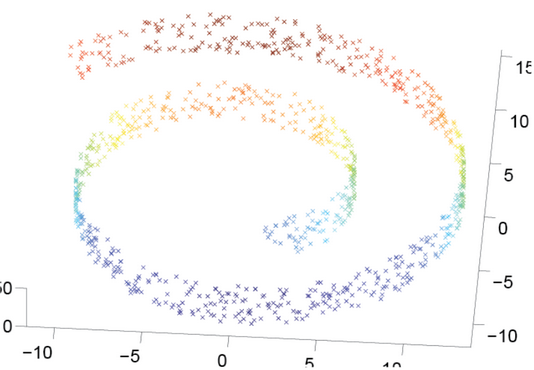
\includegraphics[width=8cm]{images/DimRed/non-linear-manifold.png}
    \caption{The ‘Swiss Roll’ dataset. 2D manifold embedded in 3D space.}
    \label{fig:non-linear-manifold}
\end{figure}

\subsubsection{Autoassociative Neural Networks (Autoencoders)}
An autoencoder is a combination of two Neural Networks: an encoder and a decoder. The train is based on reconstruction loss and provides a low-dimensional representation.

The structure is a neural network with a reduced size of hidden layers which learn to reconstruct their input by minimizing a loss function.
\begin{figure}[H]
    \centering
    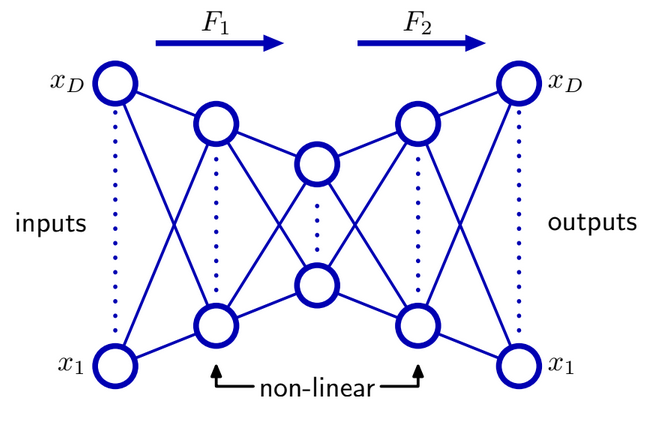
\includegraphics[width=8cm]{images/DimRed/autoencoder.png}
    \caption{A basic autoencoder example.}
    \label{fig:non-linear-manifold}
\end{figure}
It is important to have the same number of neurons in input and output.

We can also use autoencoders for image based application with Convolutional and Convolutional Transposed layers
\begin{figure}[H]
    \centering
    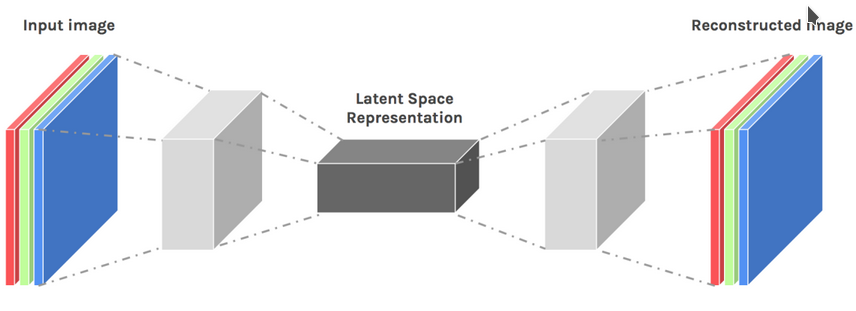
\includegraphics[width=8cm]{images/DimRed/autoencoder-image.png}
    \caption{Autoencoder for images.}
    \label{fig:non-linear-manifold}
\end{figure}
Given a dataset ${x_{n}}$, Autoencoders are trained with the same sample $x_{n}$ both in input and in output. Autoencoders learn how to encode/decode the samples in a dataset in a low-dimensional space. Autoencoders can be seen as a method for non-linear principal component analysis.

Autoencoders can be used for anomaly detection. We can teach an Autoencoder to reconstruct "good" samples and then calculate a threshold based on the final train loss found during training. We can then test samples, see if the reconstruction error is higher than the threshold and, if so, consider that sample an anomaly.

\subsection{Generative Models}
For these models, the aim is not only to reduce dimensionality, but also to use the latent space to reconstruct the input and modify it.

\textbf{Variational Auto-Encoders} (VAEs) focus on learning latent space structure\\
\textbf{Generative Adversal Networks} (GANs) focus on learning a distribution (no latent space in general)

\subsubsection{VAEs}
The goal is to modify the data in specific directions and identify meaningful directions in latent space. Some examples are face distortion, digit production and 3D mesh distortion.

\begin{figure}[H]
    \centering
    \begin{subfigure}[b]{0.45\textwidth}
        \centering
        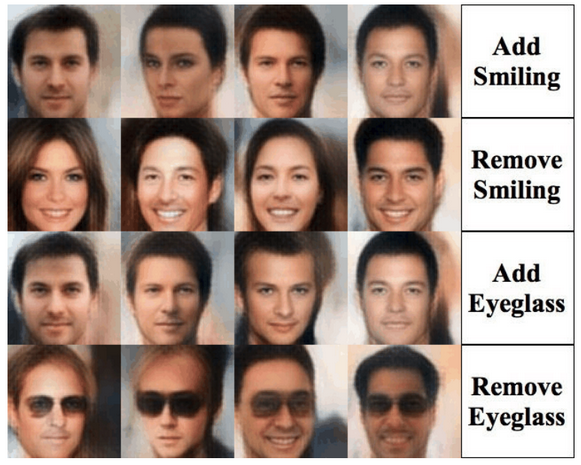
\includegraphics[width=\textwidth]{images/DimRed/vaes-1.png}
        \caption{Example of application of VAEs on faces.}
        \label{fig:vaes_1}
    \end{subfigure}
    \hfill
    \begin{subfigure}[b]{0.45\textwidth}
        \centering
        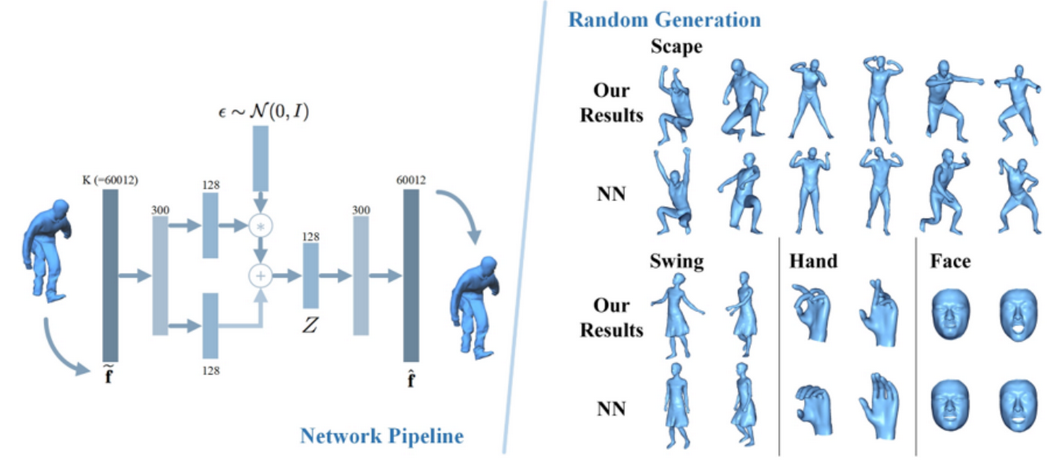
\includegraphics[width=\textwidth]{images/DimRed/vaes-2.png}
        \caption{Example of application of VAEs on 3D mesh fold.}
        \label{fig:vaes_2}
    \end{subfigure}
\end{figure}

Main idea: Encoder produces a distribution instead of a vector. Decoder operates on samples from this distribution

\begin{figure}[H]
    \centering
    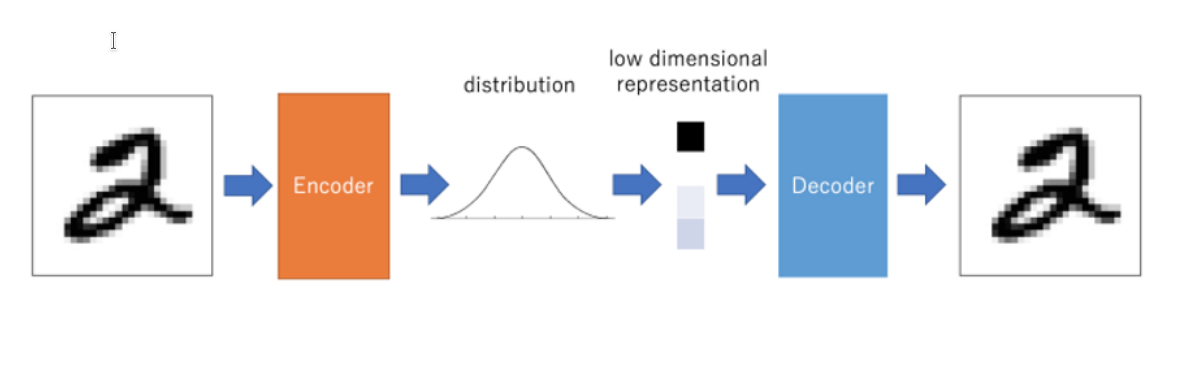
\includegraphics[width=12cm]{images/DimRed/vae.png}
    \caption{VAE architecture.}
    \label{fig:non-linear-manifold}
\end{figure}

But how do we produce a distribution? How do we prevent degeneration? We can consider a parametric distribution (typically Gaussian that produces a mean and a variance). Then we add a loss term based on the KL divergence (Evidence Lower Bound) that gives how much the distribution of the latent space differs from a standard Gaussian distribution with 0 mean and an identity covariance matrix. We also have another factor $\epsilon$ that works as a weight and regulates the strictness of the re-parametrization of the Gaussian that the VAE is learning (an high $\epsilon$ brings better looking Gaussians but worsen the reconstruction quality).

In practice, since we have a distribution, we could try to sample one value of the distribution. For instance, if we have an image and we give it to the decoder of a VAE, we get a value as output. Then, the value is processed by the Gaussian distribution and this generates a sample. This sample is then passed to the decoder who generates the output.

The sampling operation is easy to perform forward given the parameters of the Gaussian. However, if we have to compute the gradient for the backpropagation, and the sampling operation is not invertible. We then solve this problem by introducing the concept of generating a sample during backpropagation and sum this value to the output of the encoder. Since this can be treated just like a constant value, during backpropagation we know how to derive it and so we can proceed.

\subsubsection{GANs}

The main goal is to sample from the input data distribution $X$. The idea is based on inverting a CNN and use adversal training. 

A GAN firstly has an encoder that uses a CNN to process an image and transform it into a vector. Following, a Decoder receives a code and produces an image. This second element uses a "deconvolutional" operator.

What we then want to do is being able to use only the decoder so that, if we give a vector as input, it is able to reconstruct an image. The meaning of dimensionality reduction is loosing importance and what really matters is the generation of an image from a vector.

now the problem becomes: How to train the decoder to produce meaningful data? 

Adversal training is when two parts of the network are competing each other in order to find an optimal solution. In GANs, we use adversal training to improve reconstruction. A GAN is then a combination of two networks: the generator network (or decoder) and the discriminator network (or critic).

The Discriminator can take as input both  real images from the dataset and images sampled from the generator. He then has to decide if the input is a real or a fake image.

\begin{figure}[H]
    \centering
    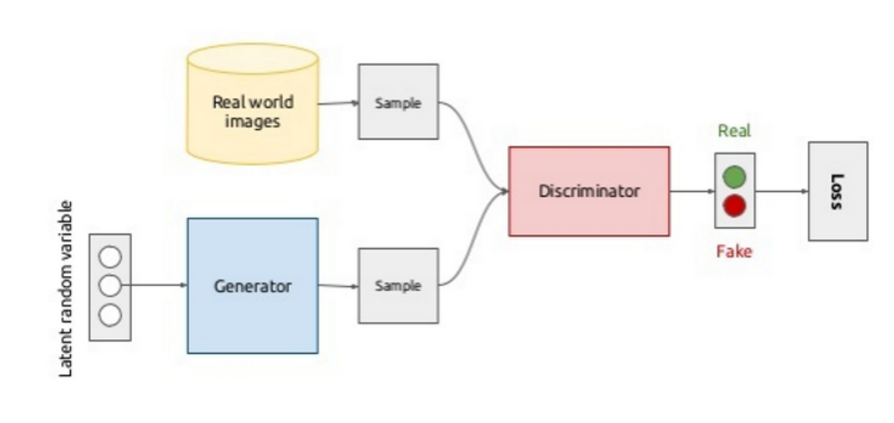
\includegraphics[width=12cm]{images/DimRed/GAN.png}
    \caption{GAN architecture.}
    \label{fig:non-linear-manifold}
\end{figure}

So, there are two roles in a GAN:
\begin{itemize}
    \item Generator produces samples of the distribution $P(X)$
    \item Discriminator identifies if a sample actually comes from the (unknown) $P(X)$ or not
\end{itemize}

during training procedure, we have the networks competing with each other:
\begin{itemize}
    \item generator tries to fool the discriminator in believing that the sample is ‘real’
    \item discriminator tries to discriminate as good as possible ‘real’ from ‘fake’ samples
\end{itemize}

and the training steps are:
\begin{enumerate}
    \item Train the discriminator by keeping the generator fixed. During this phase, images from the generator are labeled as fake because the discriminator has to learn the difference between fake and real images.
    
    \vspace{0.1cm}
    
    AKA. Train the discriminator with a batch of data $\{(x_{n}, \text{Real})\} \cup {(x_{m}', \text{Fake})}$, where $x_{n}$ comes from the data set, while $x_{m}'$ are images generated from the generator with random values of the latent variable.
    \item Train the generator by keeping the discriminator fixed. During this phase, images from the generator are labeled as real because the generator wants to fool the discriminator.
    
    \vspace{0.1cm}
    
    AKA. Train the generator by using the entire model (generator + discriminator) with discriminator layers fixed (i.e., not trainable) with a bacth of data ${(r_{k}, \text{Real})}$, where $r_{k}$ are random values of the latent variable
\end{enumerate}

What about the loss? We can notice that when the loss increases for the discriminator, it decreases for the generator and viceversa. Very often, if you plot the losses during time it will have a 2d-DNA shape that slowly decreases until they will converge. We don't want to have that one of the two losses goes to zero while the other diverges. A model is trained when the two losses converge and the accuracy of the discriminator is around 50\%. Now we can generate images from the generators that are similar to the ones from the dataset.

Additional topic: GANs can be exploited to attack ML models !!! A generative model can be defined in order to make an anomaly detection model fail.


\chapter{Reinforcement Learning}
\section{Dynamic Systems}

A dynamic system is a system that evolves during time. Until now, we didn't consider time. Now we will consider a system that also considers time and, in particular, discrete time.

\begin{figure}[H]
    \centering
    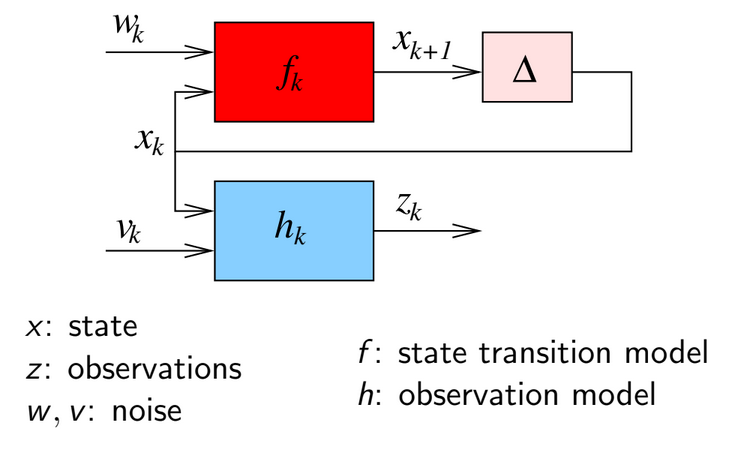
\includegraphics[width=12cm]{images/Reinforcement Learning/dynam_sys.png}
    \caption{Taxonomy ao a dynamic system}
    \label{fig:dyn_sys}
\end{figure}

An important step in the dynamic system \ref{fig:dyn_sys} is $X_{k}$ which is the snapshot f how is the situation at this moment, while $X_{k + 1}$ is the snapshot at the next timestep. The evolution can be represented by a list of snapshots: $X_{1}, X_{2}, \dots, X_{t}$. The state transmission model $f_{k}$ is the function that evolves the system. This function models how the state changes between steps. In this picture, the input variables that influences this function are not shown. However they are implicitly represented inside the noise $W_{k}$. We have another important model which is the observation model $h_{k}$. $z_{k}$ are the observations created by the observation model. $\Delta$ is an offset in time that gives to the model consideration of time.

\subsection{Reasoning vs learning in Dynamic Systems}
For \textbf{reasoning}, we have the model $(f, h)$ (Input) and the current state $x_{k}$, so we can predict the future $(x_{k + T}, z_{k + T})$. In \textbf{learning} we have the past experience $(z_{0:k})$ (Input) and we want to determine the model $(f, h)$.

\subsection{State of a Dynamic System}

The staet $x$ encodes:
\begin{itemize}
    \item all the past knowledge needed to predict the future
    \item the knowledge gathered through operation
    \item the knowledge needed to pursue the goal
\end{itemize}

When the state is fully observable, the decision making problem for an agent is to decide which action must be executed in a given state. The agent has to compute the function:
\begin{equation}
    \pi : X \xrightarrow{} A
\end{equation}
The goal of the agent is to learn a function $\pi$ that maps states to actions.

If we want to compare Reinforcement Learning and Supervised learning, we can point out that:
\begin{itemize}
    \item Supervised learning tries to learn a function $f : X \xrightarrow{} Y$, given $D = \{x_{i}, y_{i}\}$
    \item Reinforcement learning tries to learn a function $\pi : X \xrightarrow{} A$, given\\ 
    $D = \{ \langle (x_{1}, a_{1}, r_{1}), \dots, (x_{n}, a_{n}, r_{n}) \rangle \}^{(i)}$
\end{itemize}
where $x_{i}$ is the $i$-th state, $a_{i}$ is the $i$-th action and $r_{i}$ is the $i$-th reward. Notice that in a RL dataset we have any combination of states, actions and rewards.

\subsection{Dynamic System Representation}

$X$: set of states
\begin{itemize}
    \item \textbf{explicit discrete and finite representation} $X = \{x_{1}, \dots, x_{n}\}$
    \item continuous representation $X = F(\dots)$ (state function)
    \item probabilistic representation $P(X)$ (probabilistic state function)
\end{itemize}
$A$: set of actions
\begin{itemize}
    \item \textbf{explicit discrete and finite representation} $A = \{xa_{1}, \dots, a_{n}\}$
    \item continuous representation $A = U(\dots)$ (control function)
\end{itemize}
$\delta$: transition function
\begin{itemize}
    \item deterministic / non-deterministic / \textbf{probabilistic}
\end{itemize}
$Z$: set of observations
\begin{itemize}
    \item explicit discrete and finite representation $Z = \{xz_{1}, \dots, z_{n}\}$
    \item continuous representation $Z = \zeta(\dots)$ (observation function)
    \item probabilistic representation $P(Z)$ (probabilistic observation function)
\end{itemize}

\subsection{Markov property}

The Markov property states that: 
\begin{itemize}
    \item Once the \textbf{current state is known}, the evolution of the dynamic system does \textbf{not depend} on the \textbf{history} of states, actions and observations.
    \item The \textbf{current state contains all the information needed} to predict the future.
    \item \textbf{Future} states are \textbf{conditionally independent} of past states and past observations given the current state.
    \item The knowledge about the current state makes past, present and future observations statistically independent.
\end{itemize}

A Markov process is a process that has the Markov property

\subsection{Markov Decision Process (MDP)}
Markov processes for decision making. \\
States are fully observable, no need of observations. \\
Graphical model:

\begin{figure}[H]
    \centering
    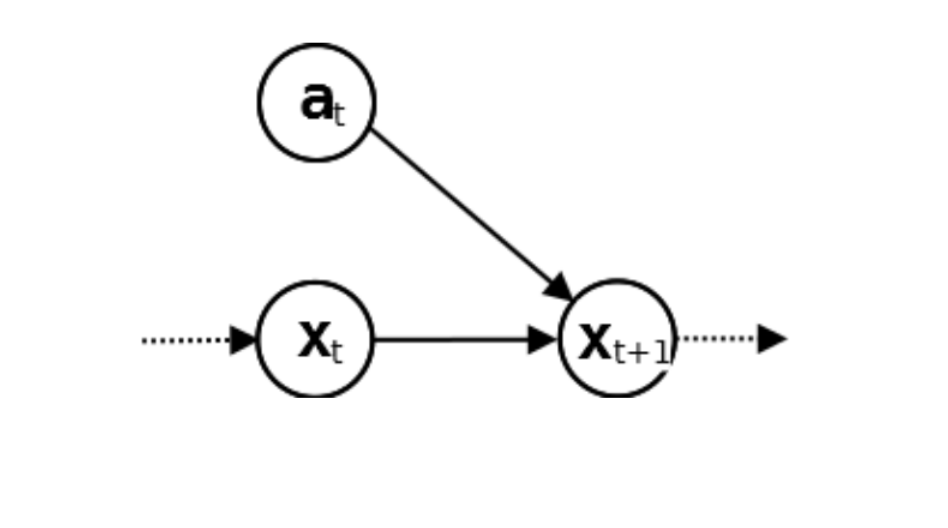
\includegraphics[width=8cm]{images/Reinforcement Learning/mdp.png}
    \caption{MDP graphical model}
    \label{fig:mdp}
\end{figure}

\section{Markov Decision Process (MDP)}
It is a decision process based on subsequent actions that makes the model evolve during time.
\subsection{Deterministic transaction}
\begin{equation}
    MDP = \langle X, A, \delta, r\rangle
\end{equation}
where $X$ is a finite set of states, $A$ is a finite set of actions, $\delta : X \times A \xrightarrow{} A$ is a transition function and $r : X \times A \xrightarrow{} \mathcal{R}$ is a reward function.

The Markov property states that $x_{t+1} = \delta(x_{t}, a_{t})$ and $r_{t} = r(x_{t}, a_{t})$. Sometimes, the reward function is defied as $r: X \xrightarrow{} \mathcal{R}$.

\subsection{Non-deterministic transaction}
\begin{equation}
    MDP = \langle X, A, \delta, r\rangle
\end{equation}
where $X$ is a finite set of states, $A$ is a finite set of actions, $\delta : X \times A \xrightarrow{} 2^{X}$ is a transition function and $r : X \times A \times X \xrightarrow{} \mathcal{R}$ is a reward function.

We have that the transition function has a set of possible alternatives:
\begin{equation*}
    \delta(x_{t}, Q_{t}) = \begin{cases}
        1\\
        x_{t+1}\\
        x_{t+4}\\
        \dots\\
        x_{t+n}\\
    \end{cases}
\end{equation*}

An example is a game of tick-tack-toe, where player has a non-deterministic view of the game as it cannot chose for his opponent.

\subsection{Stochastic transitions}
\begin{equation}
    MDP = \langle X, A, \delta, r\rangle
\end{equation}
where $X$ is a finite set of states, $A$ is a finite set of actions, $\delta$ is modeled as $P(x'|x, a)$ which is a probability distribution over transitions and $r : X \times A \times X \xrightarrow{} \mathcal{R}$ is a reward function.

\subsection{Fully observability in MDP}
States are fully observable. In presence of non-deterministic or stochastic actions, the state resulting from the execution of an action is not known before the execution of the action, but it can be fully observed after its execution.

So, non determinism means that the future is uncertain, not that the state cannot be known.

\subsection{MDP Solution Concept}
Given an MDP, we want to find an optimal policy function $\pi : X \xrightarrow{} A$. For each state $x \in X, \pi (x) \in A$ is the optimal action to be executed in such state.

\textit{optimality = maximize the cumulative reward}

Optimality is defined with respect to maximizing the (expected value of the) cumulative discounted reward. Discounted because future rewards are less valuable than current rewards (better some money today than some money tomorrow). 
\begin{equation}
    V^{\pi}(x_{1}) \equiv E[\overline{r_{1}} + \gamma\overline{r_{2}} + \gamma^{2}\overline{r_{3}} + \dots ]
\end{equation}

where $\overline{r_{t}} = r(x_{t}, a_{t}, x_{t+1})$, $a_{t} = \pi(x_{t})$, and $\gamma \in [0, 1]$ is the discount factor for future rewards.

Optimal policy: $\pi^{*} \equiv \underset{\pi}{argmax}\ V^{\pi}(x),\ \forall x \in X$. It is the policy that guarantees the maximum value of the value function overall the possible policies for every initial state.

 $V$ is called value function. We can distinguish a value function for Deterministic case and Non-deterministic / Stochastic case:
 \begin{equation}
     \text{Deterministic: } V^{\pi}(x_{1}) \equiv r_{1} + \gamma r_{2} + \gamma^{2} r_{3} + \dots
 \end{equation}
  \begin{equation}
     \text{Non-deterministic / Stochastic: }V^{\pi}(x_{1}) \equiv E[r_{1} + \gamma r_{2} + \gamma^{2} r_{3} + \dots]
 \end{equation}

 \subsubsection{Optimal Policy}

 $\pi^{*}$ is an \textbf{optimal policy} if and only if for any other policy $\pi$:
 \begin{equation}
     V^{\pi^{*}}(x) >= V^{\pi}(x), \forall x
 \end{equation}
for infinite horizon problems, a stationary MDP always has an optimal stationary policy.

\section{Reasoning and Learning in MDP}

Let's re define the difference between Reasoning and Learning by considering the MDP model. The Probelm is: MDP$\langle X, A, \delta, r \rangle$ and the solution is a policy $pi: X \xrightarrow{} A$. If the MDP$\langle X, A, \delta, r \rangle$ is completely known, we have reasoning or planning, while if it not completely known we have learning. Simple examples of reasoning in MDP can be modeled as a search problem and solved using standard search algorithm (e.g., A*).

\section{One-state Markov Decision Process}
\begin{equation}
    MDP = \langle \{x_{0}\}, A, \delta, r \rangle
\end{equation}
where $x_{0}$ is an unique state, A is a finite set of actions, $\delta(x_{0}, a_{i}) = x_{0},\ \forall a_{i} \in A$ is the transition function, $r(x_{0}, a_{i}, x_{0}) = r(a_{i})$ is the reward function. The optimal policy is $\pi^{*}(x_{0}) = a_{i}$.

We can have different configurations, based on the environment and the actions:
\begin{itemize}
    \item If $r(a_{i})$ is \textbf{deterministic} and reward function \textbf{known}, then the optimal policy is $\pi^{*}(x_{0}) = \underset{a_{i} \in A}{argmax} r(a_{i})$
    \item If $r(a_{i})$ is \textbf{deterministic} and reward function \textbf{unknown}, then what we can do is:
    \begin{enumerate}
        \item for each $a_{i} \in A$, execute the action $a_{i}$ and collect the reward $r_{i}$
        \item the optimal policy is then: $\pi^{*}(x_{0}) = a_{i}$, with $i = \underset{i=1, \dots, |A|}{argmax}\ r(i)$
    \end{enumerate}
    Note that we need $|A|$ iterations.
    \item If $r(a_{i})$ is \textbf{non-deterministic} and reward function \textbf{known}, then the optimal policy is $\pi^{*}(x_{0}) = \underset{a_{i} \in A}{argmax}\ E[r(a_{i})]$. 

    For instance, if we have that $r(a_{i}) = Gauss(\mu_{i}, \sigma_{i})$, then $\pi^{*}(x_{0}) = a_{i}$, with $i = \underset{i=1, \dots, |A|}{argmax}\ \mu_{i}$

    \item If $r(a_{i})$ is \textbf{non-deterministic} and reward function \textbf{unknown}, then what we can do is:
    \begin{enumerate}
        \item Initialize a data structure $\Theta$
        \item for each time t=1, \dots, T (until termination condition):
        \begin{enumerate}
            \item choose an action $a_{(t)} \in A$
            \item execute $a_{(t)}$ and collect the reward $r_{(t)}$
            \item update the data structure$\Theta$
        \end{enumerate}
        \item the optimal policy is then: $\pi^{*}(x_{0}) = \dots$, according to the data structure $\Theta$
    \end{enumerate}
    
    For example, if we only know that $r(a_{i}) = N(\mui_{i}, \sigma_{i})$, we can use a vector of $N$ components initialized to zero for the data structure $\Theta$ and anther data structure $c[i] \xleftarrow{} 0$, $i=1,\dots, |A|$, then at each loop, when we have to update the data structure, we increment $c[\hat{i}] += 1$ and update $\Theta_{(t)}[\hat{i}] \xleftarrow{} \frac{1}{c[\hat{i}]} \left(r_{(t)} + \left( r_{(t)} + \left( c[\hat{i}] - 1 \right) \right) \Theta_{(t-1)}[\hat{i}]\right)$.

    The optimal policy can then be computed as $\pi^{*}(x_{0}) = a_{i}$, with $i = \underset{i=1, \dots, |A|}{argmax}\ \Theta_{(T)}[i]$
\end{itemize}

\subsection{Experimentation strategies}

How can we chose actions? We have to distinguish \textbf{exploration} (select a random action) and \textbf{exploitation} (select the best action).

Two strategies are explained next.

\subsubsection{$\sigma$-greedy}
$\sigma$-greedy picks a random action with probability $\sigma$ and the best action with probability $1 - \sigma$. $\sigma$ can vary during time and be adaptive, or simply increase during time (first exploration, then exploitation)..

\subsection{soft-max strategy}
action with higher $\hat{Q}$ values are assigned higher probabilities, but every action is assigned a non-zero probability.
\begin{equation}
    P(a_{i}|x) = \frac{k^{\hat{Q}(x, a_{i})}}{\sum_{j} k^{\hat{Q}(x, a_{j})}}
\end{equation}
$k > 0$ determines how strongly the selection favors actions with high $\hat{Q}$ values. k may increase over time (first exploration, then exploitation)..


 \subsection{Learning with Markov decision processes}
 Given an agent accomplishing a task according to an $MDP\langle X, A, \delta, r \rangle$ for which functions $\delta$ and r are unknown to the agent, determine the optimal policy $\pi^{*}$. Note that this is not a supervised learning approach.

 The target function is $\pi: X \xrightarrow{} A$ but we don't have training examples $\{(x_{(i)}, \pi(x_{(i)})\}$. 

 Since $\delta$ and r are not known, the agent cannot predict the effect of its actions. But it can execute them and then observe the outcome.\\
 The learning task is thus performed by repeating these steps:
 \begin{itemize}
     \item choose an action
     \item execute the chosen action
     \item observe the results
     \item collect the reward
 \end{itemize}


\subsection{Approaches to Learning with MDP}
we have two possible approaches: \textbf{value iteration} (estimate the Value function and then compute $\pi$) and \textbf{Policy iteration} (estimate directly $\pi$)

\subsubsection{value iteration}
The agent could learn the value function $V^{\pi^{*}}(x)$ (written as $V^{*}(x)$ and determine the optimal policy from it.
\begin{equation}
    \pi^{*}(x) = \underset{a \in A}{argmax}\left[r(x, a) + \gamma V^{*}(\delta(x, a))\right]
\end{equation}
However, this policy cannot be computed in this way because $\delta$ and r are not known.

\subsubsection{Q Function}
when $\delta$ and r are not known, we need something else.
What we can do is use $Q^{\pi}(x, a)$, which is the expected value when executing a in the state x and then act according to $\pi$. So it says how good is to execute $a$ from $x$.
\begin{equation}
    Q^{\pi}(x, a) \equiv r(x, a) + \gamma V^{\pi}(\delta(x, a))
\end{equation}
\begin{equation}
    Q^{*}(x, a) \equiv r(x, a) + \gamma V^{*}(\delta(x, a))
\end{equation}
If the agent learns Q, then it can determine the optimal policy without knowing $\delta$ and $r$.
\begin{equation}
    \pi^{*}(x) = \underset{a \in A}{argmax}\ Q(x, a)
\end{equation}

let's consider the \textbf{deterministic transition}. Observe that
\begin{equation}
    V^{*}(x) = \underset{a \in A}{max}\{r(x, a) + \gamma V^{*}(\delta(x, a))\} = \underset{a \in A}{max} Q(x, a)
\end{equation}
thus we can rewrite:
\begin{equation}
    Q(x, a) \equiv r(x, a) + \gamma V^{*}(\delta(x, a))
\end{equation}
as
\begin{equation}
    Q(x, a) \equiv r(x, a) + \gamma \underset{a \in A}{max} Q(\sigma(x, a), a')
\end{equation}

The \textbf{training rule} is:
\begin{equation}
    \hat{Q}(x, a) \xleftarrow{} \overline{r} + \gamma \underset{a'}{max}\hat{Q}(x', a')
\end{equation}
both the reward and the next state are given by the environment.

The \textbf{algorithm} is then:
\begin{itemize}
    \item initialize the Q table with all 0.
    \item observe the current state
    \item foreach $t = 1, \dots, T$ until termination condition:
    \begin{itemize}
        \item chosse an action a
        \item execute the action a
        \item observe the new state $x'$
        \item collect the immediate reward $\overline{r}$
        \item update the qtable:
        \begin{equation}
            \hat{Q}_{t}(x, a) \xleftarrow{} \overline{r} + \gamma \underset{a'}{max}\hat{Q}_{t-1}(x', a')
        \end{equation}
    \end{itemize}
    \item optimal policy: 
    \begin{equation}
        \pi^{*}(x) = \underset{a \in A}{argmax}\ \hat{Q}_{T}(x, a)
    \end{equation}
\end{itemize}

\textbf{Property}: $\hat{Q}_{n}(x, a)$ underestimates $Q_{n}(x, a)$ and we have that $0 \leq \hat{Q}_{n}(x, a) \leq \hat{Q}_{n + 1}(x, a) \leq Q(x, a)$. Convergence is guaranteed if all state-action pairs visited infinitely often. This means that every state must always have a probability of being visited (exploration). A way of doing this is by choosing action a with an uniform distribution. We can also use $\sigma$-greedy or softmax probability.


Lets now consider the \textbf{non deterministic} case: the reward and transition funcions are non deterministic. This means that the same action may give different results. What we do is to use the expected values in $V$ and $Q$:
\begin{equation}
    V^{\pi}(x) \equiv E[r_{t} + \gamma r_{t + 1} + \gamma^{2} r_{t+2} + \dots] = E[\sum_{i = 0} ^ {\inf}\gamma^{i} r_{t + i}]
\end{equation}
optimal policy:
\begin{equation}
    \pi^{*} \equiv \underset{\pi}{argmax}\ V^{\pi}(x),(\forall x)
\end{equation}

Q is defined as:
\begin{equation}
    Q(x, a) \equiv E[r(x, a) + \gamma V^{*}(\gamma(x, a))] = \dots = E[r(x, a)] + \gamma \sum_{x'} P(x'|x, a)\underset{a'}{max}\ Q(x', a')
\end{equation}

\textbf{properties}:
\textbf{Deterministic Q-learning does not converge in non-deterministic worlds}. But Non-deterministic Q-learning also converges when every pair state, action is visited infinitely often

\subsection{Evaluating RL Agents}

Cumulative reward plot may be very noisy. A better approach could be:

Repeat until termination condition:
\begin{itemize}
    \item Execute k steps of learning
    \item Evaluate the current policy $\pi_{k}$ (average and stddev of cumulative reward obtained in d runs with no exploration)
\end{itemize}

\subsection{Different RL algorithms}
\begin{itemize}
    \item \textbf{Temporal Difference (TD)} learning
    \item \textbf{SARSA}
\end{itemize}

\subsection{k-armed bandit}
we have a single state and k actions. Each action returns a reward s.t. $r(a_:{i}) = N(\mu_{i}, \sigma_{i})$ Gaussian distriubution. 
train rule (same for non-deterministic Q learning):
\begin{equation}
    Q_{n}(a_{i}) \xleftarrow{} Q_{n-1} (a_{i}) + \alpha [\overline{r} - Q_{n - 1} (a_{i})]
\end{equation}
\begin{equation}
    \alpha = \frac{1}{1 + v_{n - 1}(a_{i})}
\end{equation}

\section{HMM and POMDP}

\subsection{Markov chain}

Dynamic system evolving according to the Markov property.
\begin{figure}[H]
    \centering
    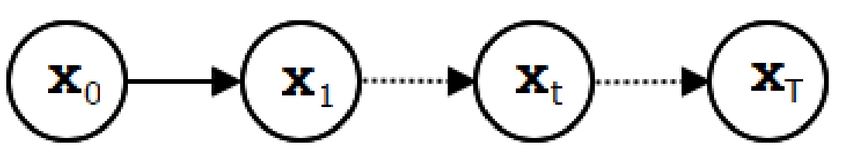
\includegraphics[width=12cm]{images/Reinforcement Learning/markov_chain.png}
    \caption{A Markov chain}
    \label{fig:markov chain}
\end{figure}
Future evolution depends only on the current state $x_{t}$

\subsection{Hidden Markov Models (HMM)}

\begin{figure}[H]
    \centering
    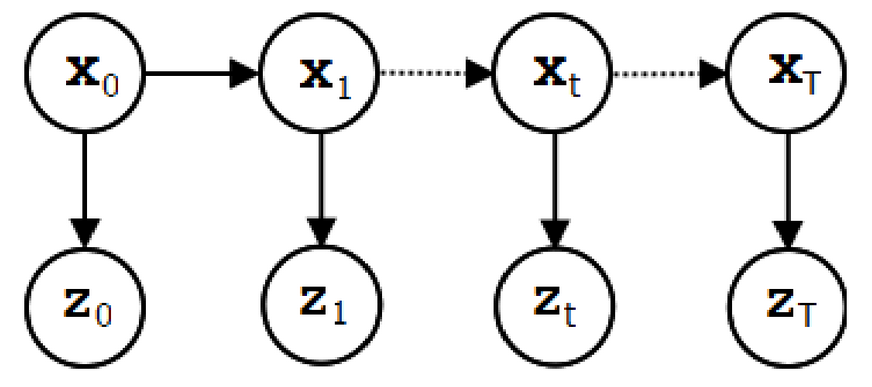
\includegraphics[width=12cm]{images/Reinforcement Learning/hmm.png}
    \caption{An Hidden Markov Model draw}
    \label{fig:hmm}
\end{figure}
states $x_{t}$ are discrete and non-observable, observations (emissions) $z_{t}$ can be either discrete or continuous. Controls $u_{t}$ are not present (i.e., evolution is not controlled by our system).


\textbf{In general}, I cannot observe the state variables $x$, but I can observe the observations $z$ which depends on the observations.

It is a Markov model because is a Markov chain and is hidden because we cannot observe the real state.

\subsubsection{Formal definition}
HMM $= \langle X, Z, \pi_{0} \rangle$ where
\begin{itemize}
    \item transition model: $P(x_{t}|x_{t-1})$
    \item observation model: $P(z_{t}|x_{t})$
    \item initial distribution: $\pi_{0}$
\end{itemize}

the state transition matrix $A = \{A_{ij}\}$
\begin{equation}
    A_{ij} \equiv P(x_{t} = j | x_{t - 1} = i)
\end{equation}

Observation model (discrete or continuous):
\begin{equation}
    b_{k}(z_{t}) \equiv P(z_{t} | x_{t} = k)
\end{equation}
Initial probabilities:
\begin{equation}
    \pi_{0} = P(x_{0})
\end{equation}

\subsubsection{HMM properties and formulae}

We apply the chain rule on HMM:
\begin{equation}
    P(x_{0:T}, z_{0:T}) = P(x_{0})P(x_{1}|x_{0})P(z_{1}|x_{1})P(x_{2}|x_{1})P(z_{2}|x_{2})\dots
\end{equation}

Given a series of observations, we want to determine the distribution over states at some time stamp. Concretely, we want to determine $P(X_{x}|z_{1},z_{2},\dots,z_{n})$. The task is called filtering if $t=n$, smoothing if $t<n$
Given HMM $= \langle X, Z, \pi_{0} \rangle$,
\begin{itemize}
    \item \textbf{Filtering}: $P(x_{T} = k | z_{1:T}) = \frac{\alpha_{T}^{k}}{\sum_{j}\alpha_{T}^{j}}$
    \item \textbf{Smoothing}: $P(x_{t} = k | z_{1:T}) = \frac{\alpha_{t}^{k}\beta^{k}_{t}}{\sum_{j}\alpha_{t}^{j} \beta^{j}_{t}}$
\end{itemize}
where:
\begin{itemize}
    \item forward iterative steps to compute
        \begin{equation}
            \alpha^{k}_{t} \equiv P(x_{t} = k, z_{1:t})
        \end{equation}
        \begin{itemize}
            \item for each state k do: $\alpha^{k}_{0} = \pi_{0}b_{k}(z_{0})$
            \item for each time $t = 1, \dots, T$ do:
            \begin{itemize}
                \item for each state k do:
                \begin{equation}
                    \alpha^{k}_{t} = b_{k}(z_{t}) \sum_{j} \alpha_{t-1}^{j}A_{jk}
                \end{equation}
            \end{itemize}
        \end{itemize}
        
    \item Backward iterative steps to compute
        \begin{equation}
            \beta^{k}_{t} \equiv P(z_{t+1:T}| x_{t} = k)
        \end{equation}
        \begin{itemize}
            \item for each state k do: $\beta^{k}_{T} = 1$
            \item for each time $t = T-1, \dots, 1$ do:
            \begin{itemize}
                \item for each state k do:
                \begin{equation}
                    \alpha^{k}_{t} = \sum_{j} \beta_{t+1}^{j}A_{jk}b(z_{t+1})
                \end{equation}
            \end{itemize}
        \end{itemize}
\end{itemize}


\subsubsection{learning in HMM}

Given output sequences, determine maximum likelihood estimate of the parameters of the HMM (transition and emission probabilities).

\begin{itemize}
    \item \textbf{Case 1}: states can be observed at training time. Note, we are assuming that during training we can see the model. In this case transition and observation models can be estimated with statistical analysis.
    \begin{figure}[H]
        \centering
        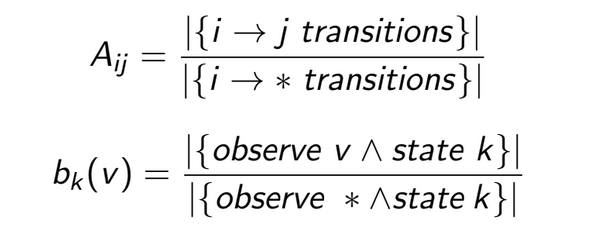
\includegraphics[width=12cm]{images/Reinforcement Learning/case1hmm.png}
        \label{fig:case1hmm}
    \end{figure}

    \item \textbf{Case 2}: states cannot be observed at training time. in this case compute a local maximum likelihood with an Expectation-Maximization (EM) method.
\end{itemize}

\subsection{POMDP agent}

Combines decision making of MDP and non-observability of HMM. We are introducing actions in HMM and we cannot observe states like in MDP.

\begin{figure}[H]
    \centering
    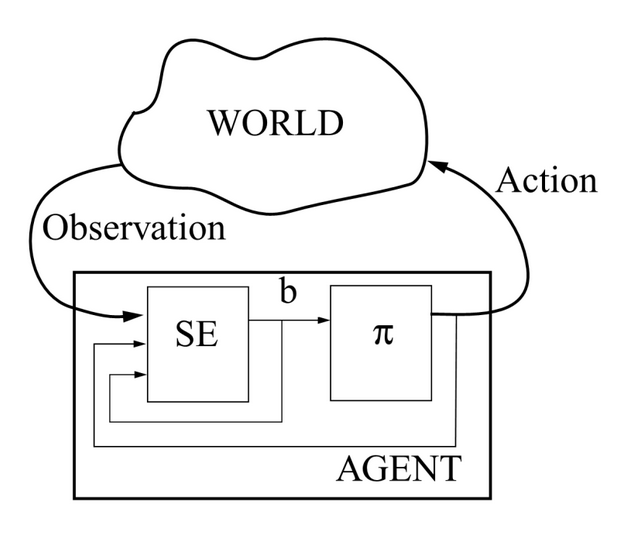
\includegraphics[width=12cm]{images/Reinforcement Learning/POMDP.png}
    \label{fig:pomdp}
\end{figure}

the POMDP representation is $POMDP = \langle X, A, Z, \delta, r, o\rangle$:
\begin{itemize}
    \item X is a set of states
    \item A is a set of actions
    \item Z is a set of observations
    \item $P(x_{0})$ is a probability distribution of the initial state
    \item $\delta(x, a, x') = P(x'|x, a)$ is a probability distribution over transitions
    \item r(x, a) is a reward function
    \item $o(x', a, z') = P(z'|x', a)$ is a probability distribution over observations.
\end{itemize}

the solution of the model is a policy (which is a functions from states to actions like in MDP), but we do not know the states.
The solution can then be a function that maps a set of observations to an action. however is difficult to learn a function that maps observations to actions as observations are potentially infinite. What we can add is the concept of \textbf{belief} of observation.

\subsection{Belief MDP}
we can add concept of belief and learn a function from belief space to actions space.
Belief $b(x) =$ probability distribution over the states. POMDP can be described as an MDP in the belief states, but belief states are infinite.
The set of possible belief is \textbf{exponential} wrt the number of states.

It is possible to transform the POMDP into an MDP, but it is not practical as it moves the model in a very complex space. However there are methods that approximates an MDP. We can use parametric models or piecewise linears to approximate the real transformation and make the POMDP algorithm more efficient.









\end{document} % ends the document
